%
% Zusammenfassung Communication Networks D-ITET
% ===========================================================================
% Author:			Marco Dober
% Version:			0.1
% Last changed: 	19.02.2019	
% ---------------------------------------------------------------------------

\documentclass[a4paper, fontsize=8pt, landscape, DIV=1]{scrartcl}
\usepackage{lastpage}
\usepackage{hyperref}
\usepackage[graphicx]{realboxes}
% Include general settings and customized commands
%
% General packages and settings
% ===========================================================================
% Author:			Silvano Cortesi (cortesis@student.ethz.ch)
% Version:			1.2
% Last changed:		03.01.2018
%
% ---------------------------------------------------------------------------




\usepackage[german]{babel} %choose your language \usepackage[german]{babel}
%\usepackage[T1]{fontenc}
\usepackage[utf8]{inputenc}
\usepackage{fancyhdr}
%\usepackage{lastpage}
%\usepackage{lmodern}
\usepackage{enumerate}
%\usepackage{float} % for positioning of figures
\usepackage[landscape, margin=1cm]{geometry}
\usepackage[dvipsnames]{xcolor}
\usepackage{pdfpages}


%% Math %%
\usepackage{todonotes}
\usepackage{amscd}
\usepackage{blindtext}
\usepackage{enumitem}
\usepackage{multicol}
\usepackage{parskip}
\usepackage{empheq}
\usepackage{amsmath}
\usepackage{amsfonts}
\usepackage{amssymb}
\usepackage{amsthm}
%\usepackage{dsfont}
%\usepackage{esint} % provides \oiint
\usepackage{mathrsfs}
%\usepackage{trfsigns}
%\numberwithin{equation}{subsection}
%\usepackage{numprint}

%% Graphics & Charts %%
\usepackage{graphicx}
%\usepackage{pdfpages}
%\usepackage{booktabs}
\usepackage{array}
%\usepackage{paralist}
%\usepackage{framed}
%\usepackage{trfsigns}
\usepackage{tikz}
%\usepackage[lofdepth,lotdepth]{subfig}
%\usepackage{tikz}  %Graphen zeichnen
%\usetikzlibrary{decorations.pathmorphing}
%\usetikzlibrary{arrows.meta,arrows}
%\usepackage{pgfplots}
%% General Settings %%
%\setlength{\parindent}{0px}
%\setkomafont{captionlabel}{\normalfont\bfseries}
\usepackage{wrapfig}
\usepackage{color,soul}

%\pagestyle{fancy}
%\lfoot{\tiny \today}
%\rfoot{\thepage\  / \pageref{LastPage}}
%\cfoot{}
%\renewcommand{\footrulewidth}{0.4pt}

%% provides command \uline{} for underlining words
%\usepackage{ulem}

%% colour headings
%\usepackage{color}
%\definecolor{bluen}{cmyk}{1,0.5,0,0}
%\definecolor{bloodorange}{cmyk}{0,.92,1,.2}
%\addtokomafont{section}{\color{bloodorange}}
%\addtokomafont{subsection}{\color{bloodorange}}
%\addtokomafont{subsubsection}{\color{bloodorange}}
%\addtokomafont{paragraph}{\small\color{bloodorange}}
%\addtokomafont{subparagraph}{\small\color{bloodorange}}

%% Signs & Special Formating %%
%\usepackage{ulem} %normalem: \emph{Text} is italic again.
%\usepackage{multicol,multirow}
%\usepackage{tabularx}
%\usepackage{stackrel}
%\usepackage{makeidx}
%\usepackage{mparhack} % bessere margiale bei seitenumbruch

% make document compact
\usepackage[compact]{titlesec}
\titlespacing{\section}{0pt}{*0}{*0}
\titlespacing{\subsection}{0pt}{*0}{*0}
\titlespacing{\subsubsection}{0pt}{*0}{*0}

\parindent 0pt
\pagestyle{empty}
\setlength{\unitlength}{1cm}
\setlist{leftmargin = *}

%include also newer PDF
% \pdfminorversion=6

% Set the color of your style
% Avaiable are: Apricot, Aquamarine, Bittersweet, Black, Blue, blue, BlueGreen, BlueViolet, BrickRed, Brown, BurntOrange, CadetBlue, CarnationPink, Cerulean, CornflowerBlue, Cyan, Dandelion, DarkOrchid, Emerald, ForestGreen, Fuchsia, Goldenrod, Gray, Green, GreenYellow, JungleGreen, Lavender, ... (more at: http://en.wikibooks.org/wiki/LaTeX/Colors)
\def\StyleColor{MidnightBlue}

%
% General commands
% ===========================================================================
% Author:			Silvano Cortesi (cortesis@student.ethz.ch)
% Version:			1.2
% Last changed:		03.01.2018
%
% ---------------------------------------------------------------------------

%..ROEMISCHE_ZAHLEN
	\newcommand{\Roe}[1]{\uppercase\expandafter{\romannumeral #1 }}

%..ZAHLENMENGEN
	\newcommand{\N}{\mathbb{N}}
	\newcommand{\Z}{\mathbb{Z}}
	\newcommand{\Q}{\mathbb{Q}}
	\newcommand{\R}{\mathbb{R}}
	\newcommand{\real}{\R}
	\newcommand{\C}{\mathbb{C}}
	\newcommand{\complex}{\C}
	\newcommand{\0}{\mathbb{O}}
	\newcommand{\F}{\mathbb{F}}
	\newcommand{\K}{\mathbb{K}}
    \newcommand{\angstrom}{\textup{\AA}}
    
%..PFEILE
	\renewcommand{\leadsto}{\Longrightarrow}
	\newcommand{\leftrightleadsto}{\Longleftrightarrow}

%..SCHRIFT
	\newcommand{\mbf}[1] {\mathbf{#1}}
	\newcommand{\mrm}[1] {\mathrm{#1}}
  \renewcommand{\phi}{\varphi}

%..VEKTOREN
	\newcommand{\Ul} {\underline}
	\newcommand{\vEx} {\vec{e}_x}
	\newcommand{\vEy} {\vec{e}_y}
	\newcommand{\vEz} {\vec{e}_z}
	\newcommand{\vEq} {\vec{e_1}}
	\newcommand{\vEw} {\vec{e_2}}
	\newcommand{\vEe} {\vec{e_3}}
	\newcommand{\transpose} {^{\text{T}}}
	\newcommand{\vect}[1]{\boldsymbol{#1}}
	
%..MATRIX
    \newcommand{\MATR}[1]{ \displaystyle \left[ \begin{matrix} #1 \end{matrix} \right]}
    \newcommand{\MATRABS}[1]{ \displaystyle \left| \begin{matrix} #1 \end{matrix} \right|}


%..KOMPLEXE ZAHLEN
	\renewcommand{\Re}{\text{Re}\,}
	\renewcommand{\Im}{\text{Im}\,}

%..OPERATOREN
	\DeclareMathOperator{\grad}{grad}
	\renewcommand{\div}{\text{div}\,}
    	\DeclareMathOperator{\rot}{rot}
    	\DeclareMathOperator{\divg}{div}
    	\DeclareMathOperator{\Tr}{Tr}
    	\DeclareMathOperator{\const}{const}
	\DeclareMathOperator{\imag}{i}
	\newcommand{\Lapl}{\hbox{\footnotesize{$\Delta$}}}

%..DIFFERENTIALRECHNUNG
	\newcommand{\Dx} {\,\mathrm{d}}
	\newcommand{\abl}[1] {\frac{\mathrm{d}}{\mathrm{d}#1}}
	\newcommand{\Abl}[2] {\frac{\mathrm{d}#1}{\mathrm{d}#2}}
	\newcommand{\ablq}[1] {\frac{\mathrm{d^2}}{\mathrm{d}#1^2}}
	\newcommand{\Ablq}[2] {\frac{\mathrm{d^2}#1}{\mathrm{d}#2^2}}
	\newcommand{\pabl}[1] {\frac{\partial}{\partial#1}}
	\newcommand{\pablq}[1] {\frac{\partial^2}{\partial#1^2}}
	\newcommand{\Pabl}[2] {\frac{\partial#1}{\partial#2}}
	\newcommand{\Pablq}[2] {\frac{\partial^2#1}{\partial#2^2}}

%..INTEGRALRECHNUNG
	\newcommand{\dint}{\displaystyle{\int}}
	\newcommand{\intab}{\int^b_a}
	\newcommand{\intinf}{\int_{-\infty}^\infty}
  \newcommand{\Int}{\int\displaylimits}
	\newcommand{\dintab}{\displaystyle{\int^b_a}}
	\newcommand{\dintpi}{\displaystyle{\int^{\pi}_{-\pi}}}
	\newcommand{\dintzpi}{\displaystyle{\int^{2\pi}_{\mbox{-}2\pi}}}
	\newcommand{\dA}{\hspace{4pt}\mathrm{d}A}
	\newcommand{\dx}{\hspace{4pt}\mathrm{d}x}
	\newcommand{\dy}{\hspace{4pt}\mathrm{d}y}
	\newcommand{\dz}{\hspace{4pt}\mathrm{d}z}
	\newcommand{\dr}{\hspace{4pt}\mathrm{d}r}
	\newcommand{\ds}{\hspace{4pt}\mathrm{d}s}
	\newcommand{\dS}{\hspace{4pt}\mathrm{d}S}
	\newcommand{\dt}{\hspace{4pt}\mathrm{d}t}
	\newcommand{\dm}{\hspace{4pt}\mathrm{d}m}
	\newcommand{\dk}{\hspace{4pt}\mathrm{d}k}
	\newcommand{\dl}{\hspace{4pt}\mathrm{d}l}
	\newcommand{\du}{\hspace{4pt}\mathrm{d}u}
	\newcommand{\dv}{\hspace{4pt}\mathrm{d}v}
	\newcommand{\dV}{\hspace{4pt}\mathrm{d}V}
	\newcommand{\dphi}{\hspace{4pt}\mathrm{d}\varphi}
	\newcommand{\domega}{\hspace{4pt}\mathrm{d}\omega}
	\newcommand{\dvarsigma}{\hspace{4pt}\mathrm{d}\varsigma}
	\newcommand{\dtau}{\hspace{4pt}\mathrm{d}\tau}
	\newcommand{\dtheta}{\hspace{4pt}\mathrm{d}\vartheta}
	\newcommand{\dmu}{\hspace{4pt}\mathrm{d}\mu}
	\newcommand{\dxi}{\hspace{4pt}\mathrm{d}\xi}
	\newcommand{\deta}{\hspace{4pt}\mathrm{d}\eta}
	\newcommand{\dvecl}{\hspace{4pt}\mathrm{d}\vec{l}}
	\newcommand{\dvecS}{\hspace{4pt}\mathrm{d}\vec{S}}

%..LIMES
    \DeclareMathOperator{\limni}{\lim\limits_{n\to\infty}}
    \DeclareMathOperator{\limxi}{\lim\limits_{x\to\infty}}
    \DeclareMathOperator{\limho}{\lim\limits_{h\to0}}
    \newcommand{\limxai}[1]{\ensuremath{\lim\limits_{x\to #1}}}

%..SUMMEN
    \DeclareMathOperator{\sumni}{\sum_{n=0}^{\infty}}
    \newcommand{\sumnia}[1]{\ensuremath{\sum_{n=#1}^{\infty}}}


%..PARTIELLE ABLEITUNG
    \DeclareMathOperator{\partf}{\dfrac{\partial f}{\partial x}}
    \newcommand{\partfo}[1]{\ensuremath{\dfrac{\partial f}{\partial #1}}}
    \newcommand{\parto}[1]{\ensuremath{\dfrac{\partial }{\partial #1}}}
    \newcommand{\partt}[2]{\ensuremath{\dfrac{\partial^2 }{\partial #1\partial #2}}}
    \newcommand{\partq}[1]{\ensuremath{\dfrac{\partial^2 }{\partial #1^2}}}


%..ENUMERATION
    \newenvironment{abc}{\begin{enumerate}[(a)]}{\end{enumerate}}
    \newenvironment{cabc}{\begin{compactenum}[(a)]}{\end{compactenum}}
    \newenvironment{romanenum}{\begin{enumerate}[i.]}{\end{enumerate}}
    \newenvironment{cromanenum}{\begin{compactenum}[i.]}{\end{compactenum}}

%..FUNCTIONS
    \DeclareMathOperator{\arsinh}{arsinh}
    \DeclareMathOperator{\arcosh}{arcosh}
    \DeclareMathOperator{\artanh}{artanh}
    \DeclareMathOperator{\arcoth}{arcoth}
    \DeclareMathOperator{\arccot}{arccot}
    \DeclareMathOperator{\Arg}{Arg}
    \DeclareMathOperator{\Log}{Log}
    \newcommand{\dis}[1]{\hspace{#1cm}}
    \newcommand{\abs}[1]{\ensuremath{\left\vert#1\right\vert}}
    \newcommand{\attention}{\raisebox{-1pt}{{\makebox[1.6em][c]{\makebox[0pt][c]{\raisebox{.13em}{\small!}}\makebox[0pt][c]{\color{red}\Large$\bigtriangleup$}}}}}
    \DeclareMathOperator{\meq}{\stackrel{!}{=}}
    
%..GRAPHICS
	\newcommand{\cgraphic}[2]{\begin{center}\includegraphics[width=#1\columnwidth,keepaspectratio]{#2}\end{center}}
	\newcommand{\mgraphic}[2]{\begin{wrapfigure}{l}{#1\linewidth}\includegraphics[width=\linewidth]{#2}\end{wrapfigure}}
    
% section color box
\setkomafont{section}{\mysection}
\newcommand{\mysection}[1]{%
    \Large\sffamily\bfseries%
    \setlength{\fboxsep}{0cm}%already boxed
    \colorbox{\StyleColor!40}{%
        \begin{minipage}{\linewidth}%
            \vspace*{2pt}%Space before
            #1
            \vspace*{-1pt}%Space after
        \end{minipage}%
    }}

%subsection color box
\setkomafont{subsection}{\mysubsection}
\newcommand{\mysubsection}[1]{%
    \normalsize \sffamily\bfseries%
    \setlength{\fboxsep}{0cm}%already boxed
    \colorbox{\StyleColor!20}{%
        \begin{minipage}{\linewidth}%
            \vspace*{2pt}%Space before
             #1
            \vspace*{-1pt}%Space after
        \end{minipage}%
    }}

% highlighter
\newcommand{\hilight}[1]{\colorbox{\StyleColor}{#1}}
\newcommand{\highlighty}[1]{%
  \setlength{\fboxsep}{0pt}\colorbox{yellow!100}{\ensuremath{#1}}}

\newcommand{\highlightg}[1]{%
  \setlength{\fboxsep}{0pt}\colorbox{green!100}{\ensuremath{#1}}}

\newcommand{\highlightbg}[1]{%
   \colorbox{green!100}{$\displaystyle #1$}}  

% equation box        
\newcommand{\eqbox}[1]{\setlength{\fboxrule}{1mm}\fcolorbox{\StyleColor}{white}{\hspace{0.5em}$\displaystyle#1$\hspace{0.5em}}}

%center equationbox
\newcommand{\ceqbox}[1]{\vspace*{4pt} \begin{center}\eqbox{#1}\end{center}\vspace*{4pt}}

%change page style for header
\pagestyle{fancy}
\footskip 20pt
\rhead{Marco Dober}
\lhead{Communication Networks}
\chead{\thepage}
\cfoot{}
\headheight 17pt \headsep 10pt
\title{Communication Networks}
\author{Marco Dober}
\date{\today}


\begin{document}
	\setcounter{secnumdepth}{3} %no enumeration of sections
	\begin{multicols*}{4}
		%
		\section*{Disclaimer}
		This summary is part of the lecture ``ETH Communication Networks'' by Prof. Dr. Laurent Vanbever (FS19). It is based on the lecture. \\[6pt]
		Please report errors to \href{mailto:doberm@student.ethz.ch}{doberm@student.ethz.ch} such that others can benefit as well.\\[6pt]	
		The upstream repository can be found at \href{https://github.com/noah95/formulasheets}{https://github.com/noah95/formulasheets}
		\vfill\null
		\pagebreak
		
		\maketitle 
		\thispagestyle{fancy}
		
		\section{Overview}
		\subsection{What is a network made of?}
		Networks are composed of three basic components:
		\begin{itemize}
			\item \textbf{End-systems} $\vert$ send \& receive data $\vert$  PC,
			Server, Smartphone, car navigation
			\item \textbf{Switches/Routers} $\vert$ forward data to destination $\vert$
			vary in size and usage (home to data center)
			\item \textbf{Links} $\vert$ connect end-systems to switches and switches
			to each other $\vert$ copper, wireless, optical-fiber
		\end{itemize}
		\includegraphics[width=
		\columnwidth]{images/Overview/network_components.png}
		The internet is a network of networks. The Internet Service Providers (ISP)
		provide internet to their customers.\\
		\includegraphics[width= \columnwidth]{images/Overview/ISP.png}
		\columnbreak
		
		There exists a huge amount of \textbf{access technologies: }
		\begin{itemize}[noitemsep]
			\item \textbf{Ethernet} $\vert$ most common, symmetric (Up- and Down-stream
			same bandwidth)
			\item \textbf{DSL} $\vert$ phone lines, asymmetric (Up- and Down-stream NOT
			same bandwidth)
			\item \textbf{CATV} $\vert$ via cable TV, shared
			\item \textbf{Cellular} $\vert$ Smart phones 
			\item \textbf{Satellite} $\vert$ remote areas
			\item \textbf{FTTH} $\vert$ fiber to the home
			\item \textbf{Fibers} $\vert$ Internet backbone 
			\item \textbf{Infiniband} $\vert$ High performance computing 
		\end{itemize}
		\subsection{How is it shared?}
		So far we discussed the "last mile" of the Internet.\\
		3 must-have \textbf{requirements} of a good network topology: 
		\begin{itemize}
			\item \textbf{Tolerate failure} $\vert$ several path between src and dst.
			\item \textbf{Sharing to be feasible (praktikabel) \& cost effective }
			$\vert$ not too much links 
			\item \textbf{Adequate per-node capacity} $\vert$ not to few links 
		\end{itemize}
		The Design of the Internet is a mix of full-mesh, chain and bus which is an
		optimization of the above requirements. This topology is called a
		\textbf{switched network}.
		\vspace{-0.5cm}
		%\vspace{-\topsep}
		\begin{itemize}[noitemsep,topsep=0pt]
			\item \textcolor{ForestGreen}{Advantages:}
			\begin{itemize}
				\item \textcolor{ForestGreen}{Sharing and per-node capacity can be adapted
					to fit the network needs.}
			\end{itemize} 
			\item \textcolor{Red}{Disadvantages:}
			\begin{itemize}
				\item \textcolor{Red}{Require smart devices to perform; forwarding,
					routing, resource allocation (Zuweisung) }
			\end{itemize} 
		\end{itemize} 
		In a switched network links and switches are shared between flows.
		\includegraphics[width=
		\columnwidth]{images/Overview/link_switch_sharing.png}
		\columnbreak
		
		There exist two approaches of sharing, both are examples of statistical
		multiplexing: 
		\begin{itemize}
			\item \textcolor{red}{\textbf{Reservation}}\\
			principle: reserve needed bandwidth in advance\\
			multiplexing: at the flow-level\\
			implementation: \textbf{circuit-switching}  
			\item \textcolor{red}{\textbf{On-demand}}\\
			principle: send data when you need\\
			multiplexing: at the packet-level\\
			implementation: \textbf{packet-switching}
		\end{itemize}
		\textbf{Circuit-Switching:}
		\vspace{-0.5cm}
		\begin{itemize}[noitemsep]
			\item Relies on the Resource Reservation Protocol.
			\item The efficiency depends on how utilized the circuit is once
			established. The circuit can be mostly idle or just be used for a small amount
			of time (bad).
			\item It doesn't route around trouble 
		\end{itemize}
		\includegraphics[width=\columnwidth]{images/Overview/circuit_switching.png}
		
		\includegraphics[width=\columnwidth]{images/Overview/circuit_switching_transfer.png}
		\begin{itemize}[noitemsep]
			\item \textcolor{ForestGreen}{Advantages:}
			\begin{itemize}
				\item \textcolor{ForestGreen}{Predictable performance} 
				\item \textcolor{ForestGreen}{Simple \& fast switching (once circuit
					established)}
			\end{itemize}
			\item \textcolor{red}{Disadvantages:}
			\begin{itemize}
				\item \textcolor{red}{Inefficient if traffic is bursty or short}
				\item \textcolor{red}{Complex circuit setup/teardown (adds delay to
					transfer)}
				\item \textcolor{red}{Requires new circuit upon failure}
			\end{itemize} 
		\end{itemize}
		\columnbreak
		
		\textbf{Packet-Switching:}
		\vspace{-0.2cm}
		\begin{itemize}[noitemsep]
			\item Data transfer is done using independent packets 
			\item Since packets are not coordinated, they can clash with each other \
			\item To absorb transient overload, packet switching relies on buffers 
			\item It routes around trouble on the fly
		\end{itemize}
		
		\includegraphics[width=\columnwidth]{images/Overview/packet_switching_buffer.png}
		\begin{itemize}[noitemsep]
			\item \textcolor{ForestGreen}{Advantages:}
			\begin{itemize}
				\item \textcolor{ForestGreen}{Efficient use of resources} 
				\item \textcolor{ForestGreen}{Simpler to implement}
				\item \textcolor{ForestGreen}{Route around trouble}
			\end{itemize}
			\item \textcolor{red}{Disadvantages:}
			\begin{itemize}
				\item \textcolor{red}{unpredictable performance}
				\item \textcolor{red}{Requires buffer management and congestion (Stau)
					Control}
			\end{itemize} 
		\end{itemize}
		Packet-switching beats circuit-switching with respect to \textbf{resiliency}
		(robustness) and \textbf{efficiency}. 
		
		\includegraphics[width=\columnwidth]{images/Overview/internet_loves_packets.png}
		\newpage
		
		\subsection{How is it organized?}
		The Internet has a hierarchical structure and consists of about 60'000
		networks: 
		\begin{itemize}[noitemsep]
			\item \textbf{Tier-1} (international)
			\begin{itemize}
				\item have no provider 
				\item $\approx$12 networks
			\end{itemize}
			\item \textbf{Tier-2} (national)
			\begin{itemize}
				\item provide transit to Tier-3s
				\item have at least one provider 
				\item $\approx$1'000s networks 	
			\end{itemize}
			\item \textbf{Tier-3} (local)
			\begin{itemize}
				\item do not provide any transit
				\item have at least one provider
				\item 85-90\% 
			\end{itemize}
		\end{itemize}
		\includegraphics[width=\columnwidth]{images/Overview/hirarchy.png}
		Some networks have an incentive (Anreiz) to connect directly, to reduce
		their bill with their own provider (direct traffic flow between them). This is
		known as \textcolor{Blue}{\textbf{peering}}\par
		
		\textbf{IXPs} (Internet Exchange Points): provide Internet connection for
		Tier2 and other providers. Only have
		\textcolor{Blue}{\textbf{peering-connections}} . 
		\includegraphics[width=\columnwidth]{images/Overview/IXPs.png}
		\subsection{How does communication happen?}
		Use \textbf{protocols} to enable communication between processes in
		different networks. Protocols are like a conversation convention. There are
		thousands of different protocols. Subdivide in different \textbf{layers} to keep
		stuff simple (Modularity).
		\begin{center}
			\textbf{5 Layer Model}\\
			\Rotatebox{270}{
				\begin{tabular}{l l l l l}
					& Layer & service provided & role & protocol \\
					\hline						
					L5& Application  & network access & exchanges \textbf{messages} btw.
					proc. & HTTP, SMTP, FTP, SIP, ...  \\ 
					\hline 
					L4& Transport & end-to-end delivery & transport \textbf{segments} btw.
					end-sys.&TCP, UDP, SCTP \\ 
					\hline 
					L3& Network  & global best-effort delivery& move \textbf{packets} around
					the network&IP \\ 
					\hline 
					L2& Link & local best effort delivery& move \textbf{frames} across a
					link& Ethernet, Wifi, DSL, LTE,... \\ 
					\hline 
					L1& Physical & physical transfer bits & move \textbf{bits} across medium
					& copper, fiber, coax, ...\\ 
				\end{tabular}
			}
		\end{center}
		\par 
		Each layer provides a service to the layer above by using the layer below.
		Physical is foundation and everything is then built on top. 
		%\includegraphics[width=\columnwidth]{images/Overview/clock.png}
		Each layer has a \textbf{unit of data} and is implemented with different
		protocols and technologies (HW/SW). We can see shift to more HW because of
		speed. 
		\includegraphics[width=\columnwidth]{images/Overview/hw_sw.png}
		Each layer takes message from above and encapsulates with its own
		\textbf{header} and/or \textbf{trailer}. 
		\includegraphics[width=\columnwidth]{images/Overview/header_adding.png}
		\begin{itemize}[noitemsep]
			\item \textbf{Switches} act as a \textbf{L2 gateway}
			\item \textbf{Routers} act as a \textbf{L3 gateway}
		\end{itemize}
		
		\subsection{How do we characterize the network?}
		We characterize the network with:
		\begin{itemize}[noitemsep]
			\item \textbf{Delay}	
			\item \textbf{Loss}
			\item \textbf{Throughput} 
		\end{itemize}
		\textbf{Delay}
		\vspace{-0.2cm}
		\begin{itemize}[noitemsep]
			\item[$\rightarrow$] transmission $\vert$ link property
			\item[$\rightarrow$] propagation $\vert$ link property
			\item[$\rightarrow$] processing $\vert$ traffic $\vert$ mostly tiny
			\item[$\rightarrow$] queuing $\vert$ traffic $\vert$ hardest to evaluate
			\begin{itemize}
				\item[$-$] arrival rate at the queue
				\item[$-$] transmission rate of outgoing link
				\item[$-$] traffic burstiness 
			\end{itemize}
			$\text{traffic intensity} = \dfrac{L\cdot a}{R}$\\
			$a = \text{average packet arrival rate [packet/sec]} $\\
			$R = \text{transmission rate of outgoing link [bit/sec]} $\\
			$L = \text{fixed packet length [bit]} $	
		\end{itemize}
		\textbf{Loss}\\
		If the buffer of a queue is full, it drops packets and hence the packets are
		lost.\par
		\textbf{Throughput}\\
		To compute throughput one has to consider the bottleneck link
		\includegraphics[width=\columnwidth]{images/Overview/traffic_intensity.png}
		As technology improves , throughput increases \& delays are getting lower,
		except for propagation $\rightarrow$ content delivery networks move content
		closer to you (e.g. akamai).
		\includegraphics[width=\columnwidth]{images/Overview/akamai.png}
		\newpage 
		
		\section{Concepts}
		\subsection{Routing}
		How do you guide \textbf{IP packet}s from a source to a destination? \\
		Like an envelope, packets have a \textcolor{LimeGreen}{\textbf{header}} and a
		\textcolor{Orange}{\textbf{payload}}.\\ 
		\begin{center}
			\includegraphics[height=0.4\columnwidth]{images/Concepts/IP_packet.png}
		\end{center}
		Routers forward IP packets \textbf{hop-by-hop}. Routing is mostly not
		symmetrical (to/back not the same). Routers locally look up their
		\textbf{forwarding table} to know where to send the packet. Forwarding decisions
		necessarily depend on the \textbf{destination}, but also can depend on others
		(source, input port).\\
		In addition to data-plane routers also have a control plane consisting of:
		\vspace{-0.2cm}
		\begin{itemize}[noitemsep]
			\item Routing
			\item Configuration
			\item Statistics
			\item ... 
		\end{itemize}  
		\textbf{Routing} is the control-plane process that \textbf{computes} and
		\textbf{populates} the forwarding tables.
		\begin{center}
			
			\includegraphics[height=0.4\columnwidth]{images/Concepts/control_data_plane.png}
		\end{center}
		\textbf{Forwarding vs. Routing}\\
		\vspace{0.1cm}	
		
		\includegraphics[width=\columnwidth]{images/Concepts/forwarding_vs_routing.png}
		A global forwarding state is valid if and only if:
		\begin{itemize}[noitemsep]
			\item No dead ends
			\item No loops
		\end{itemize} 
		
		\subsubsection{Verifying that a forwarding state is valid}
		It's easy to verify that a routing state is valid. \\
		Simple algorithm: 
		\vspace{-0.1cm}
		\begin{enumerate}[noitemsep]
			\item Mark all outgoing ports with an arrow
			\item Eliminate all link with no arrow 
			\item Sate is valid iff the remaining graph is a \textbf{spanning-tree}
		\end{enumerate} 
		See the following pictures for an example with a resulting spanning tree and
		one with no spanning tree, hence no valid forwarding state.
		\includegraphics[width=\columnwidth]{images/Concepts/check_s_t.png}
		
		\subsubsection{How to compute forwarding states}\label{kap:How to compute
			forwarding}
		Producing valid routing state is harder $\rightarrow$ prevent dead ends
		(easy) \& loops (hard). Prevent loops is the hard part, this is where routing
		protocols differ. There are three ways to compute valid routing state: 
		\begin{enumerate}[noitemsep]
			\item Use tree-like topologies $\vert$ \textbf{Spanning-tree}
			\item Rely on a global network view $\vert$ \textbf{Link-state}
			\item Rely on distributed computation $\vert$ \textbf{Distance vector} 
		\end{enumerate}
		In the Internet we use 3., because it is not possible to make precise map of
		whole Internet.\\
		In Networks we use 2.\\
		Inside (part of) Networks we use 1. \par
		
		\textbf{1. Spanning Tree}\\
		The easiest way to avoid loops is to route traffic in a loop free topology
		(Sherlock). Simple algorithm: 
		%\vspace{-0.2cm}
		\begin{enumerate}[noitemsep]
			\item Take an arbitrary topology
			\item Build a spanning tree and ignore all other links
			\item Done!
		\end{enumerate}
		It works, because spanning trees only have one path between any two nodes.
		There are numerous tress for a topology and they vary in efficiency. \\
		Once we have an spanning tree, forwarding is easy $\rightarrow$ just
		\textbf{flood} the packets everywhere (see picture below). This is very
		\textbf{inefficient}. 
		\includegraphics[width=\columnwidth]{images/Concepts/flooding_1.png}
		Solution: Nodes can \textbf{learn} how to reach nodes by remembering where
		packets came from. Ethernet works just like that. Learning is
		\textbf{topology-dependent!}\\
		Routing by flooding on a spanning tree (in a nutshell):
		\begin{itemize}[noitemsep]
			\item Flood first packet to node you're trying to reach\\ $\rightarrow$ all
			switches learn where you are
			\item When destination answers, some switches learn where it is\\
			$\rightarrow$ some because packet to you is not flooded anymore
			\item The decision to flood or not is done on each switch\\ $\rightarrow$
			depending on who has communicated before 
		\end{itemize}
		\begin{itemize}[noitemsep]
			\item \textcolor{ForestGreen}{Advantages:}
			\begin{itemize}
				\item \textcolor{ForestGreen}{Plug-and-Play (no config. needed)} 
				\item \textcolor{ForestGreen}{Automatically adapts to moving host}
			\end{itemize}
			\item \textcolor{red}{Disadvantages:}
			\begin{itemize}
				\item \textcolor{red}{Mandate a spanning tree (eliminate many links form
					the topology)}
				\item \textcolor{red}{Slow to react to failures / host movements}
			\end{itemize} 
		\end{itemize}
		
		\textbf{2. Link-state}\\
		If \textbf{each routers} knows the entire graph, it can \textbf{locally}
		compute paths to all other nodes. Once a node \textit{u} knows the entire
		topology, it can compute shortest paths using \textbf{Dijkstra's algorithm}:
		\includegraphics[width=\columnwidth]{images/Concepts/Dijkstra.png}
		$u$ is the node running the algorithm\\
		$c(u,v)$ is the weight of the link connecting $u$ and $v$. \\
		$D(v)$ is the smallest distance currently known by $u$ to reach $v$.\\
		\includegraphics[width=\columnwidth]{images/Concepts/Dijkstra_example.png} 
		Normally the algorithm has $\mathcal{O}(n^2)$ complexity ($n$ being the
		number of nodes), but with the help of a heap (data-structure...) the complexity
		can be brought down to $\mathcal{O}(n\log n)$, which is really
		\textbf{efficient}.\\
		From the shortest paths, $u$ can directly compute its forwarding table! 
		\includegraphics[width=\columnwidth]{images/Concepts/forwarding_table.png}
		
		\textbf{How do we know cost?}\\
		Initally, routers only knwo their ID and their neighbors and the cost to
		reach them. They then build message known as Link-state (with neighbors and
		their cost/weight) and flood it in the network\\
		$\rightarrow$ At the end of the flooding process everyone should have the
		exact same view of the network. \\
		I can configure wight of links \textbf{static} by hand (Dijkstra will
		converge), or \textbf{dynamic} (may be problematic).\par 
		
		\textbf{3.Distance-vector}\\
		Paths can be computed in distributed computation.\\
		Let $d_x(y)$ be the cost of the least-cost path known by $x$ to reach $y$.
		\\
		Each node bundles these distances into one message (vector) that it
		\textbf{repeatedly} sends to all its neighbors. \\
		Each node updates its distances based on neighbors vectors:\\
		$d_x(y)=\min\{c(x,v)+d_v(y)\}$, overall neighbors $v$.\\
		This leads to a recursive computation of the shortest path, the result
		must be the same as Dijkstra algorithm! 
		Example: Compute shortest path from $u$ to D:\\
		$d_u(D)=\min\{c(u,A)+d_A(D), c(u,E)+d_E(D)\}$\\
		$\downarrow$\\
		$d_A(D)=\min\{c(A,B)+d_B(D), c(A,C)+d_C(D)\}=\min\{2+1,1+4\}=3$\\
		$\downarrow$\\
		$d_E(D)=\min\{c(E,C)+d_C(D), c(E,G)+d_G(D),c(E,u)+d_u(D)\}=5$\\
		$\downarrow$\\
		$d_u(D)=\min\{3+d_A(D), 2+d_E(D)\}=6$\\
		As before $u$ can directyl infer its forwarding table, by directing the
		traffic to its best neighbor (the one which advertises the smallest cost).
		Evaluating the complexity of DV is harder. 
		
		\subsection{Reliable delivery}\label{Subsec:Reliable_Delivery}
		How do you ensure reliable transport on top of best-effort delivery?\\
		\textbf{Goals:}
		\begin{itemize}[noitemsep]
			\item Keep the network simple,dumb\\
			$\rightarrow$ make it easy to build/operate network
			\item Keep application as network unaware as possible\\
			$\rightarrow$ Developer should focus on app, not network 
		\end{itemize}
		\textbf{Design:}
		\begin{itemize}
			\item Implement reliability in-between, in the networking stack\\
			$\rightarrow$ relive the burden from both the app and network
		\end{itemize}
		The Internet puts \textbf{reliability in L4}, just above the network
		layer.\\
		What can the mean Internet do to our IP-packets:
		\begin{itemize}[noitemsep]
			\item Lost or delayed
			\item Corruption
			\item Reordering
			\item Duplication 
		\end{itemize}
		We have four goals of reliable transfer:
		\begin{itemize}[noitemsep]
			\item \textbf{Correctness:} ensure data is delivered, in order, and
			untouched
			\item \textbf{Timeliness:} minimize time until data is transferred 
			\item \textbf{Efficiency:} optimal use of bandwidth
			\item \textbf{Fairness:} play well with concurrent communications  
		\end{itemize}
		\textbf{Correctness:}\\
		A reliable transport design is correct iff:\\
		A packet is \textcolor{Red}{always resent} if the previous packet was lost
		or corrupted. A packet may be resent at other times.\\
		Note: It is \textcolor{Red}{ok to give} up after a while, but it must be
		announced to the application.\par
		
		Designing a \textcolor{Red}{correct}, \textcolor{Red}{timely},
		\textcolor{Red}{efficient} transport mechanism knowing that packets can get
		\textcolor{Red}{lost} (focus on mentioned aspects):
		\includegraphics[width=\columnwidth]{images/Concepts/send_packet.png} 	 
		There is a clear tradeoff between timeliness and efficiency in the
		selection of the timeout value. Big challenge to choose optimal value.\\
		Small timers: Risk of \textbf{unnecessary retransmissions}\\
		Large timers: Risk of \textbf{slow transmission} \par
		
		To improve timeliness just send multiple packets at the same time and not
		wait to ACK every packet. \\
		Approach: 
		\begin{itemize}[noitemsep]
			\item Add sequence number to every packet
			\item Add buffers to sender and receiver: 
			\begin{itemize}
				\item[$-$] Sender: store packets sent \& not acknowledged
				\item[$-$] Receiver: store out-of-order packets received
			\end{itemize}
		\end{itemize} 
		\includegraphics[width=\columnwidth]{images/Concepts/packets_wo_ack.png} 	
		
		One problem that can occur is: 
		
		\includegraphics[width=\columnwidth]{images/Concepts/packets_wo_ack_problem.png}
		
		To solve this issue  we need a mechanism for \textcolor{Red}{\textbf{flow
				control}}.
		Using a \textbf{sliding window} is one way to do that:
		\begin{itemize}
			\item[$-$] Sender keeps a list of the sequence \# it can send.\\
			$\rightarrow$ known as the \textit{sending window}
			\columnbreak
			\item[$-$] Receiver keeps a list of acceptable sequence \#\\
			$\rightarrow$ known as the \textit{receiving window }
			\item[$-$] Sender and receiver negotiate the window size\\
			$\rightarrow$ sending window $\le$ receiving window
		\end{itemize} 
		Example with a window-size of 4 packets:
		\includegraphics[width=\columnwidth]{images/Concepts/windowsize4_1.png} 
		%\vspace{0.2cm}
		Window after sender receives \textcolor{Red}{ACK 4 }
		%\vspace{0.1cm}
		\includegraphics[width=\columnwidth]{images/Concepts/windowsize4_2.png} 
		Timeliness of the window protocol depends on the size of the sending
		window.\par
		
		\textbf{ACKing individual packets}
		\vspace{-0.2cm}
		\begin{itemize}[noitemsep]
			\item \textcolor{ForestGreen}{Advantages:}
			\begin{itemize}
				\item \textcolor{ForestGreen}{Know fate of each packet} 
				\item \textcolor{ForestGreen}{Simple window algorithm}
				\item \textcolor{ForestGreen}{Not sensitive to reordering}
			\end{itemize}
			\item \textcolor{red}{Disadvantages:}
			\begin{itemize}
				\item \textcolor{red}{Unnecessary retransmission upon losses}
			\end{itemize} 
		\end{itemize}
		
		\textbf{Cumulative ACKs}\\
		ACK the highest sequence number for which all the previous packets have
		been received.
		\vspace{-0.2cm}
		\begin{itemize}[noitemsep]
			\item \textcolor{ForestGreen}{Advantages:}
			\begin{itemize}
				\item \textcolor{ForestGreen}{Recover from lost ACKs}
			\end{itemize}
			\item \textcolor{red}{Disadvantages:}
			\begin{itemize}
				\item \textcolor{red}{Causes unnecessary retransmissions}
				\item \textcolor{red}{Confused by reordering}
				\item \textcolor{red}{Incomplete information about which packets have
					arrived}
			\end{itemize} 
		\end{itemize}
		
		\textbf{Full information feedback}\\
		List all packets that have been received highest cumulative ACK, plus any
		additional packets
		\vspace{-0.2cm}
		\begin{itemize}[noitemsep]
			\item \textcolor{ForestGreen}{Advantages:}
			\begin{itemize}
				\item \textcolor{ForestGreen}{Complete information}
				\item \textcolor{ForestGreen}{Resilient (belastbar) form of individual
					ACKs}
			\end{itemize}
			\item \textcolor{red}{Disadvantages:}
			\begin{itemize}
				\item \textcolor{red}{Overhead}
			\end{itemize} 
		\end{itemize}
		
		With individual ACKs and full information detection of a missing packet is
		easy (implicit/explicit). \\
		With cumulative ACKs missing packets are harder to know. \par
		
		\textbf{Fairness:}\\
		Fair is mostly not efficient. Defining what fair is, is not easy. What
		matters is to \textbf{avoid starvation}. Equal-per-flow is good enough for this.
		Simply dividing available bandwidth doesn't work.\\
		We want to give users with small demands what they want and evenly
		distribute the rest. \textbf{max-min fair allocation} is such that: the lowest
		demand is maximized $\rightarrow$ the second lowest is maximized $\rightarrow$
		the third lowest is maximized and so on...\\
		\textbf{max-min fair allocation:}
		\begin{enumerate}[noitemsep]
			\item Start with all flows at rate 0
			\item Increase the flows until there is a new bottleneck in the network
			\item Hold the fixed rate of the flows that are bottlenecked
			\item Got to step 2 for the remaining flows. 	 
		\end{enumerate}  
		Max-min fair allocation can be approximated by increasing window until a
		loss is detected. \par
		
		\textbf{Corruption:}\\
		Dealing with corruption is easy: Rely on a checksum and treat corrupted
		packets as lost ones. \par 
		
		\textbf{Reordering:}\\
		Effect depends on ACKing mechanism which is used:\\
		$\bullet$ Individal ACK: \textcolor{ForestGreen}{no problem}\\
		$\bullet$ Full feedback: \textcolor{ForestGreen}{no problem}\\
		$\bullet$ Cumm. ACKs: \textcolor{Red}{Create duplicate ACKs}.\par
		
		\textbf{Duplicates:}\\
		Can lead to duplicated ACKs whose effect depends on the ACKing mechanism:
		\\
		$\bullet$ Individual ACK: \textcolor{ForestGreen}{no problem}\\
		$\bullet$ Full feedback: \textcolor{ForestGreen}{no problem}\\
		$\bullet$ Cumm. ACKs: \textcolor{Red}{problematic}\par
		
		\textbf{Delay:}\\
		Can create useless timeouts for all designs. It is hard to deal with the
		different delays which occur over the whole network. How do I set the right
		amount of timeout?\\
		\newpage
		
		\section{The Link Layer}
		\subsection{What is a link?}
		\textbf{Link =  Medium + Adapter}\\
		Network adapters communicate together through the medium.\\
		In the link layer we talk about \textbf{Frames} which are sent form one
		adapter to the other.\\
		\includegraphics[width=\columnwidth]{images/Link_Layer/link.png} 
		\textbf{Sender}
		\vspace{-0.3cm}
		\begin{itemize}[noitemsep]
			\item Encapsulate packets in a frame
			\item add error checking bits, flow control,...
		\end{itemize}
		\textbf{Receiver:}
		\vspace{-0.3cm}
		\begin{itemize}[noitemsep]
			\item Look for errors, flow control,...
			\item Extract packet and passes it to network layer 
		\end{itemize}
		Link-Layer provides a best effort delivery service to the network layer,
		composed od \textbf{5} sub services.
		\begin{itemize}[noitemsep]
			\item \textbf{Encoding} $\vert$ represents the 0's and 1's
			\item \textbf{Framing} $\vert$ encapsulates packet into a frame
			(header/trailer)
			\item \textbf{Error detection} $\vert$ detects errors with checksum
			\item \textbf{error correction} $\vert$ optionally correct errors
			\item \textbf{Flow Control} $\vert$ pace sending and receiving node 
		\end{itemize} 
		
		\subsection{How do we identify link adapters?}
		\textbf{M}edium \textbf{A}ccess \textbf{C}ontrol address:
		\vspace{-0.2cm}
		\begin{itemize}[noitemsep]
			\item \textbf{Identify the sender \& receiver adapters} $\vert$ used
			within a link
			\item \textbf{Are uniquely assigned} $\vert$ hard coded into adapter
			\item \textbf{Use a flat space of 48 bits} $\vert$ allocated
			hierarchically 
		\end{itemize}
		The \textcolor{Green}{first} 24 bits blocks are assigned to network
		adapter vendor by IEEE. (1 Vendor may have more than 1 block.)
		
		\includegraphics[width=\columnwidth]{images/Link_Layer/first_mac_block.png}
		The \textcolor{Orange}{second} 24 bits block is assigned by the vendor to
		each network adapter.(My use the same in geographically different locations!)
		
		\includegraphics[width=\columnwidth]{images/Link_Layer/second_mac_block.png}
		broadcast address has set all bits to 1: ff:ff:ff:ff:ff:ff, enables to
		send a frame to all adapters on the link.\\
		By default, adapters only decapsulate frames addressed to the local MAC or
		broadcast address. The promiscuous mode enables to decapsulate everything.\\
		Why don't we simply use IP-addresses?
		\begin{enumerate}[noitemsep]
			\item Links can support any protocol (not just IP) $\vert$ different
			addresses on different kind of links
			\item Adapters may move to different locations $\vert$ cannot assign
			static IP address, it has to change
			\item \textbf{Adapters must be identified during bootstrap} $\vert$ need
			to talk to an adapter to give it an IP address 
		\end{enumerate} 
		You need to solve two problems when bootstrapping an adapter:
		\begin{itemize}[noitemsep]
			\item Who am I? (How do I acquire an IP address $\vert$ MAC-to-IP
			binding) $\vert$ \textcolor{Red}{Dynamic Host Configuration Protocol DHCP}
			\item Who are you? (Given an reachable IP-address on a link, how do I
			find out what MAC to use) $\vert$ IP-to-MAC binding $\vert$
			\textcolor{Red}{Address Resolution Protocol ARP}
		\end{itemize}
		Network adapters traditionally acquire an IP address using \textbf{DHC}:
		\begin{enumerate}[noitemsep]
			\item \textbf{Discovery} $\vert$ Client searching DHCP Server (via
			broadcast)
			\item \textbf{Offer} $\vert$ DHCP server sending offer to client
			\item \textbf{Request} $\vert$ Client request IP from DHCP server
			\item \textbf{ACK} $\vert$ DHCP server assigns IP and sends ACK 
		\end{enumerate}
		\includegraphics[width=\columnwidth]{images/Link_Layer/DHCP.png}
		\par 
		
		The \textbf{ARP} enables to discover the MAC associated to an IP: 
		\begin{enumerate}[noitemsep]
			\item ARP \textbf{Request}: Who has $<$some Ip$>$ tell $<$my IP$>$ to
			broadcast MAC
			\item ARP \textbf{Reply}: $<$some IP$>$ is at $<$this MAC$>$
			\item Requester puts entry in his \textbf{ARP-table}
		\end{enumerate}
		\includegraphics[width=\columnwidth]{images/Link_Layer/ARP.png}
		
		\subsection{How do we share a network medium?}
		Some medium are \textbf{multi-access}: $>1$ host can communicate at same
		time.\\
		\textcolor{Red}{Problem: Collision lead to garbled (verstümmelt) data.}\\
		\textcolor{ForestGreen}{Solution: Distributed algorithm for sharing the
			channel.}\\
		Essentially there are three techniques to deal with Multi Access Control
		(MAC):
		\begin{itemize}[noitemsep]
			\item \textbf{Divide the channel into pieces} $\vert$ either in time or
			frequency
			\item \textbf{Take turns} $\vert$ pass a token for the right to transmit
			\item \textbf{Random access} $\vert$ allow collisions, detect them and
			then recover
		\end{itemize} 
		
		\subsection{What is Ethernet?}
		\begin{itemize}[noitemsep]
			\item Was invented as a broadcast technology
			\item Is the dominant wired LAN technology 
			\item Has managed to keep up with the speed race
		\end{itemize}
		Ethernet offers an \textbf{unreliable} and \textbf{connectionless}
		service.\\
		Unreliable:
		\begin{itemize}[noitemsep]
			\item[$-$] Receiving adapter does not acknowledge anything
			\item[$-$] Packets passed to the networks layer can have gaps
		\end{itemize}
		Connectionless: 
		\begin{itemize}[noitemsep]
			\item[$-$] No handshake between sender and receiver
		\end{itemize}
		Traditional Ethernet relies on CSMA/CD (carries-sense multiple access with
		collision detection). All hosts were on a big bus-cable connected. You needed to
		sense the cable in order to know if someone is speaking. multiple hosts had
		access to the medium, while you were speaking you still were listening to detect
		collisions. CSMA/CD imposes \textbf{limits} to the network length.\\
		$\mathrm{Network\ length}=\frac{min\ frame\ size\ \cdot\ speed\ of\
			light}{2\cdot bandwidth}$\\
		For this reason Ethernet imposes a minimum packet size of 512 bits.\\
		Modern Ethernet links interconnect exactly two hosts, in full duplex,
		rendering collisions impossible. 
		\begin{itemize}[noitemsep]
			\item CSMA/CD is only needed for half-duplex communication
			\item This means the 64 Byte restriction is not strictly needed (but
			still kept)
			\item Multiple Access Protocols are still important for wireless
			communication
		\end{itemize}
		The Ethernet header is simple, composed of 6 fields: 
		\includegraphics[width=\columnwidth]{images/Link_Layer/eth_header.png}
		Ethernet efficiency is $\approx97.5\%$ (paylod/framesize). 
		
		\subsection{How do we interconnect segments at the link layer?}
		Historically, people connected Ethernet segments together at the physical
		level with ethernet \textbf{hubs}. Hubs work by repeating bits from one port to
		all the others (flooding everything). 
		\includegraphics[width=\columnwidth]{images/Link_Layer/hub.png}
		\begin{itemize}[noitemsep]
			\item \textcolor{ForestGreen}{Advantages:}
			\begin{itemize}
				\item \textcolor{ForestGreen}{Cheap, simple}
			\end{itemize}
			\item \textcolor{red}{Disadvantages:}
			\begin{itemize}
				\item \textcolor{red}{Inefficient}
				\item \textcolor{red}{Limited ot one LAN technology}
				\item \textcolor{red}{Limited number of nodes/distances} 
			\end{itemize} 
		\end{itemize}
		LANs are now almost exclusively composed of Ethernet \textbf{switches}.
		Switches connect two or more LANs together on the Link layer, actings as L2
		gateways. Switches are \textbf{store and forward} devices, they: 
		\begin{itemize}[noitemsep]
			\item Extract the DST MAC $\vert$ from the frame
			\item Look up the MAC in a table $\vert$ using exact match
			\item Forward the frame $\vert$ on the appropriate port
		\end{itemize}
		Similiar to IP routers, except they are one layer below. Switch enables
		each LAN segment to carry its own traffic (no flooding of network). 
		\includegraphics[width=\columnwidth]{images/Link_Layer/switch_network.png}
		Switches are Plug-and-Play they build their forwarding table on their
		own.\\
		The advantages of switches are numerous: 
		\begin{itemize}[noitemsep]
			\item \textcolor{ForestGreen}{Advantages:}
			\begin{itemize}
				\item \textcolor{ForestGreen}{Only forward frames where needed} $\vert$
				avoids unnecessary load on segments
				\item \textcolor{ForestGreen}{Join segments using different
					technologies}
				\item \textcolor{ForestGreen}{Improved privacy} $\vert$ hosts can only
				snoop traffic traversing their segment
				\item \textcolor{ForestGreen}{Wider geographic span} $\vert$ separates
				segments allow longer distance
			\end{itemize} 
		\end{itemize}
		\newpage
		
		When Frames arrive:
		\vspace{-0.2cm} 
		\begin{itemize}[noitemsep]
			\item [$-$] Inspect the SRC MAC address
			\item [$-$] associate the address with the port
			\item [$-$] Store the mapping in the switch table
			\item [$-$] Launch a timer to eventually forget the mapping
		\end{itemize}
		In case of misses, switches simply flood the network (when in doubt,
		shout).\\
		When a frame arrives with an unknown DST $\rightarrow$ forward the frame
		out all ports, except where the frame arrived from.\\ 
		Flooding enables \textbf{automatic discovery} of hosts, but with loops the
		load increases exponentially! Solution: Reduce the network to one logical
		\textbf{spanning tree}.\\
		In practice, switches run distributed Spanning-Tree-Protocol
		(\textbf{STP}). \\
		Construction of a spanning tree in a nutshell: Switches...
		\begin{itemize}[noitemsep]
			\item Elect a root $\vert$ the one with the smallest identifier
			\item determine if each interface is on the shortest path from the root
			$\vert$ if not $\rightarrow$ disable it.
		\end{itemize}
		For this switches exchange Bridge Protocol Data Unit (BPDU) messages\\
		Each Switch X iteratively sends: 
		\includegraphics[width=\columnwidth]{images/Link_Layer/BPDU.png}
		Initially: 
		\vspace{-0.2cm}
		\begin{itemize}[noitemsep]
			\item Each switch proposes itself as root $\vert$ sends (X,0,X) on all its
			interfaces
			\item Upon receiving (Y,d,X), checks if Y is a better root $\vert$ if so,
			consider Y as new root, flood updated message 
			\item Switch compute their distance to the root, for each port $\vert$
			simply add 1 to the distance received, if shorter, flood
			\item Switches disable interfaces not on shortest-path
		\end{itemize}
		tie-breaking: 
		\vspace{-0.2cm}
		\begin{itemize}[noitemsep]
			\item Upon receiving $\ne$ BPDUs from $\ne$ switches with $=$ cost
			$\rightarrow$ pick the BPDU with the lower siwtch sender ID
			\item Upon receiving $\ne$ BPDUs from a neighboring switch $\rightarrow$
			Pick the BPDU with the lowest port ID. 
		\end{itemize}
		To be robust, STP must react to failures: 
		\vspace{-0.2cm}
		\begin{itemize}[noitemsep]
			\item Any switch, link or port can fail $\vert$ including the root switch
			\item Root switch continuously send messages $\vert$ announcing itself as
			the root (1,0,1), others forward it
			\item Failures are detected through timeout (soft state) $\vert$ if no
			word from root in X, times out and claims to be root 
		\end{itemize}
		\subsection{Virtual Local Aerea Networks VLANs}
		The Local Area Networks we have considered so far define single broadcast
		domains (if one broadcasts, everyone receives it).\\
		As the networks scales, operators like to \textbf{segment} thir LANs.\\
		Why?
		\begin{itemize}[noitemsep]
			\item Improves \textbf{security} $\vert$ smaller attack surface
			(visibility \& injection)
			\item Improves \textbf{performance} $\vert$ limits the overhead fo
			broadcast traffic 
			\item Improves \textbf{logistics} $\vert$ separate traffic by role (staff,
			student,...)
		\end{itemize} 
		You do not want to separate your LAN physically (huge pain), but reader do
		it in software $\rightarrow$ \textbf{Virtual} Networks.\\
		Definition:\\
		A VLAN identifies a set of ports attached to one or more Ethernet Switches,
		forming one broadcast domain. 
		\includegraphics[width=\columnwidth]{images/Link_Layer/VLAN.png}
		Switches need \textbf{configuration} tables telling them which VLANs are
		accessible via which interface.\\
		To identify VLAN, switches add \textbf{new header} when forwarding traffic
		to another switch.  
		\includegraphics[width=\columnwidth]{images/Link_Layer/VLAN_header.png}
		With VLANs, Ethernet links are divided in two sets:
		\textcolor{Blue}{\textbf{access}} and \textcolor{Red}{\textbf{trunks}} (inter
		switch) links.\\
		Trunks carry traffic for more than one VLAN (access not), there the new
		header is needed! On the access links not! Communication between VLANs goes over
		a router!
		Each switch runs one MAC learning algorithm for each VLAN.
		\begin{itemize}[noitemsep]
			\item When a switch receives a frame wit an unknown or broadcast DST.
			\begin{itemize}
				\item [$\rightarrow$]	it forwards it on all the ports that belong to the
				same VLAN
			\end{itemize}
			\columnbreak
			\item  When a switch learns a SRC address on a port
			\begin{itemize}
				\item [$\rightarrow$] it associates it to the VLAN of this port and only
				uses it when forwarding frames to this VLAN	
			\end{itemize}
		\end{itemize}
		\includegraphics[width=\columnwidth]{images/Link_Layer/trunks_access.png}
		Switches can also compute per VLAN spanning trees $\rightarrow$ distinct
		SPT for each VLAN! This enables better use of the network. 
		
		\section{The Network Layer}
		\subsection{IPv4 addresses}
		IPv4 addresses are unique 32-bits number associated to a network interface
		(on a host, router). IP addresses are usually written using dotted-quad
		notation. 
		\includegraphics[width=\columnwidth]{images/Network_Layer/IP_address.png}
		Routers forward packets based on their DST IP address. If IP addresses were
		assigned arbitrarily routers would require forwarding table entries for all of
		them!\\
		IP addresses are hierarchical, composed of a\textcolor{Red}{ prefix
			(network address)} and a \textcolor{ForestGreen}{suffix (host address)}. 
		
		\includegraphics[width=\columnwidth]{images/Network_Layer/prefix_suffix.png}
		Each prefix has a given length, usually written using the slash notation:\\
		IP prefix: 82.130.102.0/\textcolor{Red}{24}$\rightarrow$ prefix length in
		bit\\
		The suffix part can then be used to address the hosts of the network.\\
		$\bullet$The \textbf{first address} of the suffix (all zeros) is used to
		identify the \textbf{network itself}.\\
		$\bullet$ The \textbf{last address} of the suffix (all ones) is used ot
		determine the \textbf{broadcast} address.\\
		\# of hosts $= 2^{32-\#\mathrm{\textcolor{Red}{suffix}}}-2$\\
		Prefixes are also sometimes specified using an address and a \textbf{mask}.
		ANDing the address and the mask gives you the prefix. \\
		Mask: set the number of suffix bits to one, the rest zeros (from left to
		right).\\
		\includegraphics[width=\columnwidth]{images/Network_Layer/mask.png}
		Routers forward IP packets based on the network part, not the host part.
		This enables a scaling of the forwarding table. \\
		Originally there were only 5 fixed allocation sizes (classes) - known as
		classful networking. This is wasteful and leaded to IP address exhaustion.\\
		\includegraphics[width=\columnwidth]{images/Network_Layer/classes.png}
		Problem: Class C was too small, so everybody requested B\\
		Solution: Classless Inter-Domain Routing (CIDR) (1993)\\
		CIDR enables flexible division between network and host addresses. 
		\begin{itemize}[noitemsep]
			\item CIDR must specify both, the address and the mask $\vert$ classful
			was communicating this in the first address bits
			\item Masks are carried by the routing algorithms $\vert$ it is not
			implicitly carried in the address.  
		\end{itemize}
		With CIDR the maximal waste is bounded to 50\%.\\
		Today, addresses are allocated in contiguous chunks:\\ 
		\includegraphics[width=\columnwidth]{images/Network_Layer/IP_chunk.png}
		\pagebreak
		
		The allocation process of prefixes is also hierarchical:\\
		
		\includegraphics[width=\columnwidth]{images/Network_Layer/prefix_allocation.png}
		
		\subsubsection{Network Address Translation (NAT)}
		In order to be able to use more hosts than available IPv4 addresses NAT was
		introduced: 
		\begin{itemize}[noitemsep]
			\item Sharing a single public address between hosts
			\begin{itemize}
				\item[$-$] Port numbers are used to distinguish
			\end{itemize}
			\item One of the main reasons we still can use IPv4
			\begin{itemize}
				\item[$-$] Saved us from address depletion
			\end{itemize}
			\item Violates the general end-to-end principle of the Internet. 
			\begin{itemize}
				\item[$-$] A NAT box adds a layer of indirection
			\end{itemize}
		\end{itemize}
		The Internet before NAT: Every machine connected to the Internet had a
		unique IPv4 address:\\
		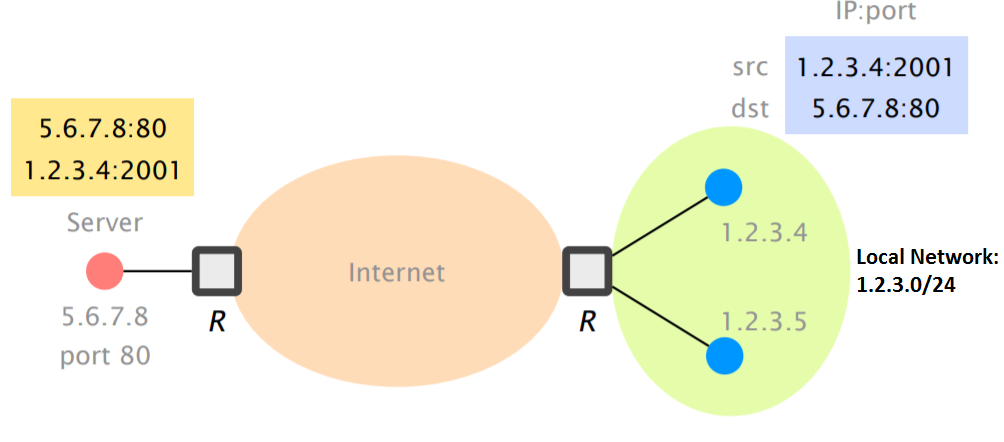
\includegraphics[width=\columnwidth]{images/Network_Layer/NAT_no.png}
		The Internet with NAT: Hosts behind NAT get a private address. The router
		works as a NAT as well and executes the translation between public and private
		addresses (NAT table). The port numbers are used to multiplex single
		addresses.\\
		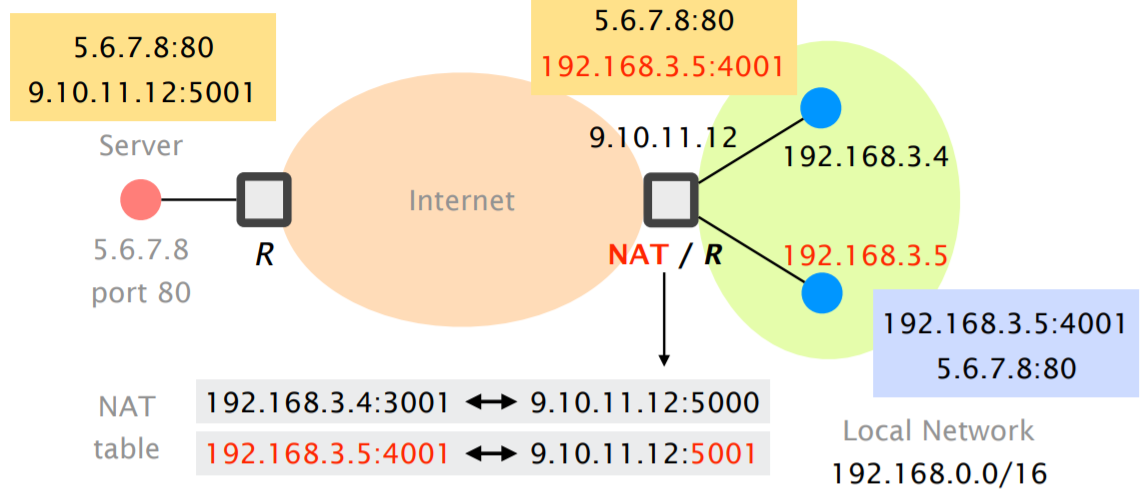
\includegraphics[width=\columnwidth]{images/Network_Layer/NAT_yes.png}
		NAT also provides other (dis-)advantages:
		\begin{itemize}[noitemsep]
			\item \textbf{Better privacy anonymization}
			\begin{itemize}
				\item[$-$] \textcolor{ForestGreen}{All hosts in one network get the same
					public IP}
				\item[$-$] \textcolor{Red}{But cookies, browser version,... still
					identifies hosts} 
			\end{itemize}
			\item \textbf{Better security}
			\begin{itemize}
				\item[$-$] \textcolor{ForestGreen}{From the outside you can not directly
					reach the hosts}
				\item[$-$] \textcolor{Red}{Problematic e.g., for online gaming} 
			\end{itemize}
			\item \textbf{Limited scalability}
			\begin{itemize}
				\item[$-$] \textcolor{Red}{Example: Wi-fi access problems in public
					places (often due to full NAT table).}
			\end{itemize}
		\end{itemize}
		
		\subsubsection{IPv4 packet}
		This is what an IPv4 Packet looks like:
		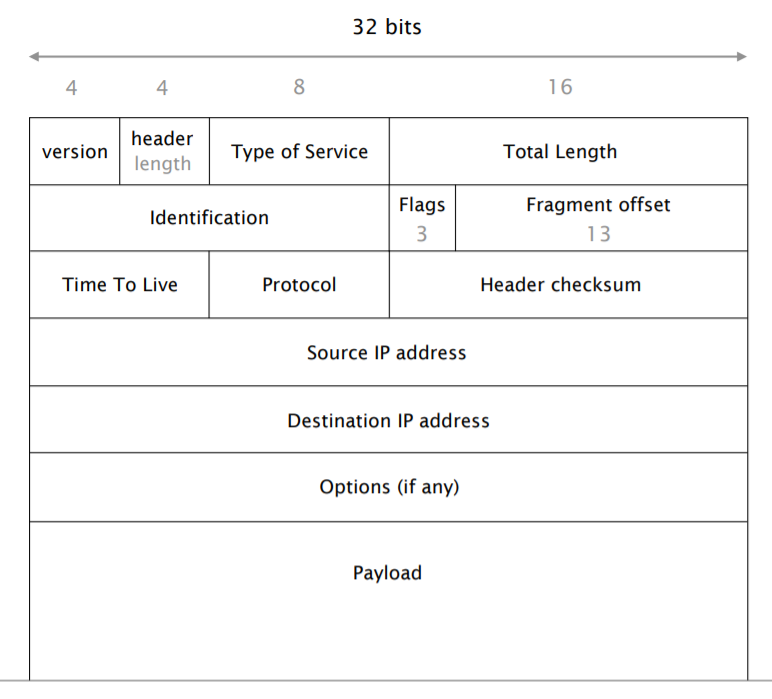
\includegraphics[width=\columnwidth]{images/Network_Layer/IPv4_packet.png}
		\textbf{Version} $\vert$  "4" or "6", tells us what other fields to
		expect\\ 
		\textbf{Header length} $\vert$ Denotes the number of 32-bits word in the
		header (typically 5 (20 Bytes)) \\ 
		\textbf{ToS} $\vert$ Allows different pakctes to be treated differently
		(low delay (VoIP), high bandwidth (Video))\\
		\textbf{Total length} $\vert$ Denotes the number of Bytes in the entire
		packet (max. 65 635, mostly 1500 because ether.)\\
		\textbf{Identification} $\vert$ Uniquely identifies the fragments of a
		particular packet.\\
		\textbf{Flag} $\vert$ Tells you if more packets are coming or not.\\
		\textbf{Fragment Offset} $\vert$ Used if need to reorder packets in right
		order.\\
		\textbf{Time To Live} $\vert$ Used to identify packets in a loop and drop
		them.\\
		\textbf{Protocol} $\vert$ Identifies the higher level protocol carried in
		the packet ("6" for TCP, "17" for UDP).\\
		\textbf{Header Checksum} $\vert$ Sum of all 16 bits words in the header
		(does not protect the payload).\\
		\textbf{Source IP} $\vert$ Uniquely identifies the Source host.\\
		\textbf{Destination IP} $\vert$ Uniquely identifies the Destination host.\\
		\textbf{Options} $\vert$ Used to provide flexibility, but mostly
		deactivated because security. (record route, strict source route, loose source
		route, timestamp, traceroute, router alert)
		
		\subsection{IPv6 addresses}
		IPv6 addresses are encoded in \textbf{128 bits}.
		\begin{itemize}[noitemsep]
			\item Notation
			\begin{itemize}
				\item[$-$] 8 groups of 16 bits each separated by a colon (:)
				\item [$-$] Each group is written as 4 hexadecimal digits
			\end{itemize}
			\item Simplification
			\begin{itemize}
				\item[$-$] Leading zeros in any group are removed
				\item[$-$] \textbf{One} section is replaced by a double colon (::).
				Normally the longest section.
			\end{itemize}
		\end{itemize}
		Examples:
		\begin{tabbing}
			1080:0:0:0:8:8000:200C:417A \= $\rightarrow$ \= 1080::8:8000:200C:417A
			\kill
			1080:0:0:0:8:8000:200C:417A \> $\rightarrow$ \> 1080::8:8000:200C:417A \\
			FF01:0:0:0:0:0:0:0101 \> $\rightarrow$ \> FF01::101 \\
			0:0:0:0:0:0:0:1 \> $\rightarrow$ \> ::1
		\end{tabbing}
		There are three types of IPv6 addresses: 
		\begin{itemize}[noitemsep]
			\item \textbf{Unicast}
			\begin{itemize}
				\item[$-$] Identifies a \textbf{single} interface
				\item[$-$] Packets are delivered to this specific interface
			\end{itemize}
			\item \textbf{Anycast}
			\begin{itemize}
				\item[$-$] Identifies a \textbf{set} of interfaces 
				\item[$-$] Packets are delivered to the \textbf{nearest} interface
			\end{itemize}
			\item \textbf{Multicast}
			\begin{itemize}
				\item[$-$] Identifies a \textbf{set} of interfaces
				\item[$-$] Packets are delivered to \textbf{all} interfaces
			\end{itemize}
		\end{itemize}
		
		\subsubsection{Unicast}
		Similar to IPv4 \textbf{global unicast} addresses are hierarchically allocated.
		Currently only \textbf{2000::/3} is used for global unicast $\rightarrow$ all
		addresses are in the range of 2000 to 3FFF.\\
		\includegraphics[width=\columnwidth]{images/Network_Layer/v6_unicast.png}
		\textbf{Link-Local} (\textcolor{Red}{\textbf{FE80}}) addresses are unique to a single link (subnet) (same as
		private IPv4 addresses). Each host/router must generate a link-local address for
		\textbf{each} of its interfaces. An interface can therefore have
		\textbf{multiple} IPv6 addresses!\\
		\includegraphics[width=\columnwidth]{images/Network_Layer/v6_link_local.png} 
		In addition to global and link-local addresses, some IPv6 uincast addresses
		have a special meaning.
		\vspace{2cm}
		\begin{itemize}[noitemsep]
			\item Unspecified address
			\begin{itemize}
				\item[$-$] 0:0:0:0:0:0:0:0
				\item[$-$] Used as src address if no IPv6 address is available
			\end{itemize}
			\item \textbf{Loopback address} 
			\begin{itemize}
				\item[$-$] ::1
				\item[$-$] 127.0.0.1 for IPv4
			\end{itemize}
			\item IPv4 embedded
			\begin{itemize}
				\item[$-$] The lowest 32 bit contain an IPv4 address. 
			\end{itemize}
			\item \textbf{Important}
			\begin{itemize}
				\item There no IPv6 broadcast addresses. 
			\end{itemize}
		\end{itemize}
		
		\subsubsection{Anycast (not in exam)}
		\begin{itemize}[noitemsep]
			\item Multiple interfaces with the same address
			\begin{itemize}
				\item[$-$] Packets are sent to the nearest interface
			\end{itemize}
			\item Anycast uses the global unicast address range
			\begin{itemize}
				\item[$-$] E.g. for DNS and HTTP services
			\end{itemize}
			\item IPv6 anycast is rarely used
		\end{itemize}
		
		\subsubsection{Multicast (not in exam)}
		Multicast addresses identify a group of receivers/interfaces. Some
		Multicast addresses are well-known and used for bootstrapping, auto-discovery,
		etc. 
		\begin{itemize}[noitemsep]
			\item FF02::1
			\begin{itemize}
				\item[$-$] All IPv6 end-systems
				\item[$-$] E.g. hosts, servers, routers, mobile devices, ... 
			\end{itemize}
			\item FF02::2
			\begin{itemize}
				\item[$-$] All IPv6 routers
				\item[$-$] All routers automatically belong to this group.
			\end{itemize}
		\end{itemize}
		
		\subsubsection{IPv6 packet header}
		\includegraphics[width=\columnwidth]{images/Network_Layer/v6_header.png}
		Compared to IPv4, IPv6 does...
		\begin{itemize}[noitemsep]
			\item \textbf{Not} include checksums in the packet header
			\begin{itemize}
				\item[$-$] link, application or transport application layer provides
				checksums
			\end{itemize}
			\item \textbf{Not} support fragmentation
			\begin{itemize}
				\item[$-$] End host is required to send small enough packets
			\end{itemize}
			\item Provide more flexibility
			\begin{itemize}
				\item[$-$] flow labels and \textbf{extension headers}
			\end{itemize}
		\end{itemize}
		\newpage 
		
		\textbf{Extension header example ICMPv6:}\\
		\includegraphics[width=\columnwidth]{images/Network_Layer/v6_extension_header.png}
		ICMPv6 can be used for \textbf{neighbor discovery} (replacement for IPv4
		ARP).\\
		First step: \textbf{neighbor solicitation}\\
		\includegraphics[width=\columnwidth]{images/Network_Layer/v6_ICMP.png}
		Second step: \textbf{neighbor advertisement}\\
		\includegraphics[width=\columnwidth]{images/Network_Layer/v6_ICMP_2.png} 	 
		
		\subsubsection{Obtain IPv6 address}
		How can a node obtain its IPv6 address(es)?
		\begin{itemize}[noitemsep]
			\item Manual configuration
			\begin{itemize}
				\item[$-$] As in the project, e.g. with ifconfig
			\end{itemize}
			\item Form a sevrer using DHCPv6
			\item \textbf{Automatically}
			\begin{itemize}
				\item[$-$] Using its link-local address and neighbor discovery
			\end{itemize}
		\end{itemize}
		
		\textbf{IPv6 configuration to find link-local address:}\\
		Consider an end-to-end system which has just started, it needs an IPv6 address to be able to send ICMPv6 messages.
		\begin{itemize}[noitemsep]
			\item MAC: 0800:200C:417A
			\item Link-local: FE80::M64(800:200C:417A)
			\begin{itemize}
				\item[$-$] M64: 64 bit representation of MAC address
			\end{itemize}
			\item Neighbor solicitation for\\ FE80::M64(800:200C:417A)
			\begin{itemize}
				\item If \textbf{no} answer, the created link-local address is valid
			\end{itemize} 
		\end{itemize}	
		\par
		
		\textbf{IPv6 autoconfiguration to obtain the IPv6 prefix of subnet:}
		\vspace{-0.2cm}
		\begin{itemize}[noitemsep]
			\item Routers periodically advertise the prefix
			\begin{itemize}
				\item[$-$] Sent to all systems: FF02::1
			\end{itemize}
			\item The advertisement can contain
			\begin{itemize}
				\item[$-$] IPv6 prefix and length
				\item[$-$] Network MTU to use
				\item[$-$] Maximum hop limit to use
				\item[$-$] Lifetime of the default router
				\item[$-$] How long generated addresses are preferred
			\end{itemize}
		\end{itemize}
		\par 
		
		\textbf{IPv6 autoconfiguration to build global unicast address:}
		\vspace{-0.2cm}
		\begin{tabbing}
			Global Unicast \= 0800:200C:417A \kill
			MAC \> 0800:200C:417A \\
			Prefix \> 2001:6a8:3080:1::/64 \\
			Global Unicast \> 2001:6a8:3080:1:M64(800:200C:417A)
		\end{tabbing}
		
		\subsubsection{From v4 to v6}
		To port your IPv4-based application to IPv6, you need to...
		\begin{itemize}[noitemsep]
			\item Change the used socket functions
			\item adjust all logging functions
			\item Adapt all data structures to support IPv6
			\item Adjust GUIs to display IPv6
		\end{itemize}
		Thats a huge pain and a big reason why it took us 20 years to make the transition from v4 to v6. Today, a lot applications and OSes use \textbf{dual stack} approach:\\
		\includegraphics[width=\columnwidth]{images/Network_Layer/dual_stack.png}
		Over the years, a lot of transition mechanisms were developed (e.g. \textbf{6in4}: Tunnel IPv6 packets over static IPv4 link). 
		
		\subsection{IP forwarding}
		Whats inside an IP router?:\\
		$\bullet$ \textbf{Data Plane:}\\
		\includegraphics[width=\columnwidth]{images/Network_Layer/data_plane.png}
		%\vspace{1cm}
		
		$\bullet$ \textbf{Control Plane:}\\
		\includegraphics[width=\columnwidth]{images/Network_Layer/control_plane.png}
		Routers maintain \textbf{forwarding entries} for each Internet prefix.\\
		When a router receives an IP packet, it performs an IP \textbf{look up} to
		find the matching prefix.\\
		CIDR makes forwarding harder, as one packet can match many IP prefixes.\\
		\includegraphics[width=\columnwidth]{images/Network_Layer/two_matches.png}
		To resolve ambiguity, forwarding is done along the \textbf{most specific}
		prefix (IF\#3)\\
		A child prefix can be \textbf{filtered} from the table whenever it shares
		the same output interface as its parent:\\
		\begin{center}
			\includegraphics[width=0.8\columnwidth]{images/Network_Layer/filtering1.png}\\
			\includegraphics[width=0.8\columnwidth]{images/Network_Layer/filtering2.png}\\
			\textcolor{Red}{Exactly the same forwarding!}
		\end{center}

		\subsection{Internet routing}
		Internet routing comes in two flavors: \textcolor{Red}{\textbf{intra}}- and
		\textcolor{ForestGreen}{\textbf{inter}}-domain routing.
		
		\includegraphics[width=\columnwidth]{images/Network_Layer/intra_vs_inter.png}
		\textcolor{Red}{\textbf{Intra}} vs. \textcolor{ForestGreen}{\textbf{Inter}}
		domain routing
		\begin{center}
			
			\includegraphics[width=0.5\columnwidth]{images/Network_Layer/intra_vs_inter_2.png}
		\end{center}
		
		\subsubsection{Intra-domain routing}
		Find paths \textbf{within} a network.\\
		Intra-domain routing enables routers to compute \textbf{good forwarding
			paths} to any internal subnet. What is \textbf{good}?\\
		\textbf{Definition:} A good path is a path that minimizes some network wide
		metric (cost, delay load, loss,...).\\
		\textbf{Approach:} Assign to each link wa weight (usually static), compute
		the \textit{shortest path} to each destination.\par
		
		\textbf{Link-state protocols}\\
		In link-state routing, routers build a precise map of the network by
		flooding local views to everyone. 
		\begin{itemize}[noitemsep]
			\item Each router keeps track of its incident links and cost $\vert$ as
			well as weather it is up or down
			\item Each router broadcast its own links state $\vert$ to give every
			router a complete view of the graph
			\item Routers run Dijkstra on the corresponding graph $\vert$ to compute
			their shortest path and forwarding table. 
		\end{itemize}
		Flooding is performed as in the L2 learning, except that it is
		\textbf{reliable}. All nodes are \textbf{ensured} to receive the latest version
		of all link-states.\\
		\newpage
		
		\begin{itemize}[noitemsep]
			\item Challanges: 
			\begin{itemize}
				\item[$-$] packet loss
				\item[$-$] out of order arrival
			\end{itemize}
			\item Solution:
			\begin{itemize}
				\item[$-$] ACK \& Retransmission
				\item[$-$] Sequence number
				\item[$-$] Time-To-Live for each link-state
			\end{itemize}
		\end{itemize}  
		A link-state node initates flooding in 3 conditions: 
		\begin{itemize}[noitemsep]
			\item \textbf{Topology change} $\vert$ link or node failure/recovery
			\item \textbf{Configuration change} $\vert$ link cost change
			\item \textbf{Periodically} $\vert$ Refresh (account for possible data
			corruption)
		\end{itemize}
		Once a node knows the entire topology, it can run Dijkstra to compute
		shortest-path.\\
		By default, link-state protocols detect changes using software based
		beaconing:\\
		Routers periodically exchange "Hello" in both directions and trigger a
		failure after few missed "Hellos". Tradeoff between: 
		\begin{itemize}[noitemsep]
			\item Detection speed
			\item Bandwidth and CPU overhead
			\item false positive/negative
		\end{itemize}  
		During network changes, the link-state database of each node might differ.
		Inconsistencies lead to transient disruptions in the form of black holes or
		loops.\\
		\textbf{Blackholes} appear due to detection delay, as nodes do not
		immediately detect failure $\rightarrow$ depends on the timeout for detecting
		lost "Hellos".\\
		\textbf{Transient loops} appear due to inconsistent link-state database.
		
		\includegraphics[width=\columnwidth]{images/Network_Layer/transient_loop.png} 
		Convergence is the process during which routers seek to actively regain a
		consistent view of the network.\\
		Network convergence time depends on 4 main factors:
		\begin{itemize}[noitemsep]
			\item \textbf{Detection}
			\begin{itemize}
				\item[$-$] realizing that a link/neighbor is down
				\item[$-$] few ms
				\item[$-$] smaller timers
			\end{itemize} 
			\item \textbf{Flooding}
			\begin{itemize}
				\item[$-$] flooding news to entire network
				\item[$-$] few ms
				\item[$-$] high-priority flooding
			\end{itemize}  
			\item \textbf{Computation}
			\begin{itemize}
				\item[$-$] recomputing Dijkstra
				\item[$-$] few ms
				\item[$-$] incremental algorithms
			\end{itemize}
			\item \textbf{Table update}
			\begin{itemize}
				\item[$-$] updating forward table
				\item[$-$] potentially \textcolor{Red}{minutes}!
				\item[$-$] better table design
			\end{itemize}
		\end{itemize} 
		The problem with updating the forwarding table is that they are flat,
		means:
		\vspace{-0.2cm}
		\begin{itemize}[noitemsep]
			\item[$-$] Entries do not share any information $\vert$ even if they are
			identical
			\item[$-$] Upon failure, all of them have to be updated $\vert$
			inefficient, but also unnecessary 
		\end{itemize} 
		The solution is to add a layer of \textbf{indirection}
		(Dereferenzierung):\\
		Replay this:\\
		
		\includegraphics[width=0.7\columnwidth]{images/Network_Layer/forward_table.png}\\
		With that:\\
		
		\includegraphics[width=\columnwidth]{images/Network_Layer/forward_table_pointer.png}
		Now we only need to update 1 entry, the one in the pointer table!
		Hierarchical tables are able to converge within 150ms \textit{independently} on
		the number of prefixes!\\
		Today, two link-state protocols are widely used:
		\vspace{1cm}
		
		\begin{itemize}[noitemsep]
			\item \textbf{OSPF}
			\begin{itemize}
				\item[$-$] used in many enterprise \& ISPs
				\item[$-$] work on top of IP
				\item[$-$] only route IPv4 by default
			\end{itemize}
			\item \textbf{IS-IS}
			\begin{itemize}
				\item[$-$] used mostly in large ISPs
				\item[$-$] work on top of link layer
				\item[$-$] network protocol agnostic
			\end{itemize}
		\end{itemize} 
		\par
		
		\textbf{Distance-vector protocols}\\
		Distance vector protocols are based on Bellman-Ford algorithm (see
		\ref{kap:How to compute forwarding} (3.))\\
		The same reasons as with the link-state cause the nodes to send new DVs.\\
		What happens when a link changes it cost?
		\vspace{-0.2cm}
		\begin{itemize}[noitemsep]
			\item Decrease cost
			\begin{itemize}
				\item[$-$] The algorithms terminates fast
				\item[$\rightarrow$] \textcolor{ForestGreen}{Good news travel fast}
			\end{itemize}
			\item Increase cost
			\begin{itemize}
				\item[$-$] The algorithm takes a while to terminate
				\item[$\rightarrow$] \textcolor{Red}{Bad news travel slow}
			\end{itemize}
		\end{itemize}
		This problem is known as \textcolor{Red}{count-to-infinity}, a type of routing
		loop.\\
		Solution: Whenever a router uses another one, it will announce it an infinite
		cost. This technique is known as \textbf{poisoned reverse}. This method does
		\textcolor{Red}{not} solve loops involving 3 or more nodes.\\
		Actual distance-vector protocols mitigate this issue by using small "infinity"
		(e.g "16").\\
		(Please see slides and exercises for examples of this problem and the solution
		method).\par
		
		\textbf{Link-state vs. Distance-vector routing:}\\
		\includegraphics[width=\columnwidth]{images/Network_Layer/state_vs_vector.png}
		
		\subsubsection{Inter-domain routing}
		Find paths \textbf{between} networks.\\
		The Internet is a network of neteorks, referred to as Autonomous Systems
		(AS). Each AS has a number which identifies it. \\
		\textbf{BGP} is the routing protocol "gluing" the entire Internet together.
		\includegraphics[width=\columnwidth]{images/Network_Layer/BGP_gluing.png}
		Using BGP, ASes exchange information about the IP prefixes they can reach,
		directly or indirectly. \\
		BGP needs to solve three key challenges:
		\begin{itemize}[noitemsep]
			\item \textbf{Scalability}
			\begin{itemize}
				\item[$-$] There is a huge \# number of networks and prefixes
				\item[$-$] 700k prefixes, $>$50k networks, millions of routers 
			\end{itemize}
			\item \textbf{Privacy}
			\begin{itemize}
				\item[$-$] Networks do not want to divulge internal topologies
				\item[$-$] Or their business relationships
			\end{itemize}
			\item \textbf{Policy enforcement}
			\begin{itemize}
				\item[$-$] Networks need to control where to send and receive traffic
				\item[$-$] without an internet-wide notion of a link cost metric
			\end{itemize}		
		\end{itemize}
		Link-state and Distance-vector do both not solve these problems, but
		\textbf{BGP} (Border Gateway Protocol) does:
		%\vspace{-0.2cm}
		\begin{itemize}[noitemsep]
			\item BGP relies on \textbf{path-vector routing} to support flexible routing
			policies and avoid count-to-infinity.
			\item BGP announcements carry \textbf{complete path} information instead of
			distances.
			\item Each AS appends itself to the path when it propagates announcements
		\end{itemize}
		Complete path information enables ASes to easily detect a loop (if they see
		themselves in the path).\\
		Each AS can apply local routing policies, each AS is free to: 
		%\vspace{-0.2cm}
		\begin{itemize}[noitemsep]
			\item Select and use any path
			\begin{itemize}
				\item[$-$]prefarably the cheapest one
			\end{itemize}
			\item Decide which path to export (if any) to which neighbor 
			\begin{itemize}
				\item preferably none to minimize carried traffic
			\end{itemize}
		\end{itemize}
		\textbf{BGP}
		\vspace{-0.2cm}
		\begin{enumerate}[noitemsep]
			\item \textbf{BGP Policies} $\vert$ Follow the money
			\item \textbf{Protocol} $\vert$ How does it work
			\item \textbf{Problems} $\vert$ Security, performance 
		\end{enumerate}
		\textbf{1. Policies}\\
		BGP is a "follow the money" protocol. Two ASes connect only if they have a
		business relationship. There are two main business relationships today: 
		\begin{enumerate}[label=(\roman*),noitemsep]
			\item Customer/Provider
			\item Peer/Peer
		\end{enumerate}
		(i) Customer/Provider\\
		Customers pays providers to get full Internet connectivity (monthly bill).\\
		The amount paid is based on peak usage, usually according to the 95\% rule.\\
		Most ISPs discount unit price of data, if you pre-commit to a certain volume
		(Mengenrabatt).\par 
		
		(ii) Peer/Peer\\
		Peers \textbf{don't} pay each other for connectivity, they do it out of
		\textbf{common interest}. $\rightarrow$ If they exchange tons of traffic, they
		save money by connecting directly to each other.\par 
		
		Follow the money:\\ 
		
		\includegraphics[width=\columnwidth]{images/Network_Layer/follow_the_money.png}
		\textcolor{ForestGreen}{Allowed}: Swisscom/Salt/Sunrise make money, without
		paying someone to provide them. $\rightarrow$ Providers transit traffic for
		their customer.\\ 
		\textcolor{Red}{Forbidden 1}: Swisscom and Deutsche get money by sending over
		ETH, the ETH network will collapse, because all the traffic will be sent over
		them. $\rightarrow$ Customer do not transit traffic between their provider.\\
		\textcolor{Red}{Forbidden 2}: Sunrise won't receive upon, but has to provide
		content over their network. $\rightarrow$ Peers do not transit traffic between
		each other.\par 
		
		These policies are defined by constraining which BGP routes are
		\textbf{selected} and \textbf{exported}.\par 
		
		\textbf{Selection}\\
		Which path to use? \textcolor{Red}{Control outbound traffic}\\
		Selection rule For a destination p, prefer routes coming from: 
		\begin{itemize}[noitemsep]
			\item Customers over 
			\item Peers over 
			\item Providers
		\end{itemize}
		There will always be a provider route, but not necessarily a customer/peer
		route.\par 
		
		\textbf{Export}\\
		Which path to advertise? \textcolor{Red}{Control inbound traffic}\\
		Route exportation:\\
		\begin{tabular}{c | c c c c} 
			&  &  & send to &  \\ 
			\hline
			&  & customer & peer & provider \\ 
			& costumer & \checkmark & \checkmark & \checkmark \\ 
			from & peer & \checkmark & - & - \\ 
			& provider & \checkmark & - & - \\ 
		\end{tabular} \\
		\vspace{-0.2cm}
		\begin{itemize}[noitemsep]
			\item  Routes coming from customers are propagated to everyone else.
			\item  Routes coming from peers and providers are only propagated to
		\end{itemize}
		\par
		
		\textbf{2. Protocol}\\
		BGP sessions come in two flavors: 
		\begin{itemize}[noitemsep]
			\item externeal BGP (\textbf{eBGP})
			\begin{itemize}
				\item[$-$] Connect border routers in different ASes
				\item[$-$] Used to learn routes to \textcolor{Red}{external destinations}\\
				
				\includegraphics[width=0.8\columnwidth]{images/Network_Layer/eBGP_session.png}
			\end{itemize}
			\item internal BGP (\textbf{iBGP})
			\begin{itemize}
				\item[$-$] Connect the routers in the same AS
				\item[$-$] Used to to disseminate (verbreiten) externally-learned routes
				internally
				\item[$-$] Routes disseminated internally are then announced externally
				again using eBGP\\ 
				
				\includegraphics[width=0.8\columnwidth]{images/Network_Layer/iBGP_session.png}
			\end{itemize}
		\end{itemize}        
		On the wire BGP is simple and only composed of four messages: 
		\begin{itemize}[noitemsep]
			\item Open 
			\begin{itemize}
				\item[$-$] establish TCP-based BGP sessions
			\end{itemize} 
			\item Notification 
			\begin{itemize}
				\item[$-$] report unusual conditions 
			\end{itemize}
			\item \textbf{Update} 
			\begin{itemize}
				\item[$-$] inform neighbor of a new best route
				\item[$-$] change in best route
				\item[$-$] removal of best route
			\end{itemize} 
			\item Keepalive
			\begin{itemize}
				\item[$-$] inform neighbor that connection is alive
			\end{itemize}
		\end{itemize}
		Update is the most important one. They carry an IP \textbf{prefix} together
		with a set of \textbf{attributes}. Attributes: 
		\begin{itemize}[noitemsep]
			\item \textbf{Next-Hop}
			\begin{itemize}
				\item[$-$] egress point identification
			\end{itemize}
			\item \textbf{AS-Path}
			\begin{itemize}
				\item[$-$] loop avoidance
				\item[$-$] outbound traffic control
				\item[$-$] inbound traffic control
			\end{itemize}
			\item \textbf{Local-Pref}
			\begin{itemize}
				\item[$-$] outbound traffic control
			\end{itemize}
			\item \textbf{Med}
			\begin{itemize}
				\item[$-$] inbound traffic control
			\end{itemize}
		\end{itemize}
		The \textbf{Next-Hop} is a global attribute which indicates where to send the
		traffic next. The Next-Hop is sent when the route enters an AS, it does not
		change within the AS. It only changes when going form one AS to an other!\\
		Solution:\\
		Force overwrite of Next-Hop to a virtual IP-address (\textbf{loopback}
		address) given to the router (unique identifier in internal network) and
		advertise this via OSPF in the internal network. Method is called
		\textcolor{Red}{\textbf{Next-Hop-Self}}.
		\includegraphics[width=\columnwidth]{images/Network_Layer/next_hop.png}
		\par 
		The \textbf{AS-Path} is a global attribute that lists all the ASes a route has
		traversed (in reverse order):\\
		\includegraphics[width=\columnwidth]{images/Network_Layer/as_path.png}
		\par 
		The \textbf{Local-Pref} is a \textit{local} attribute set at the border, it
		represents how \textit{preferred} a route is. Where do I want to send my
		traffic. Here all the routers will prefer DT over Swisscom:\\
		\includegraphics[width=\columnwidth]{images/Network_Layer/local_pref.png}
		\par 
		The \textbf{MED} is a global attribute which encodes the relative proximity of
		a prefix wrt to the announcer. You can \textbf{influence} your neighbor and try
		to tell them where to send your receiving traffic (Only works with multiple
		connections to the \textbf{same AS}). In the end though, the sender decides
		where he sends the traffic $\rightarrow$ I can influence not control:\\
		\begin{center}
			\includegraphics[width=0.7\columnwidth]{images/Network_Layer/med.png}
		\end{center}
		\par 
		Each BGP router processes updates according to a precise \textbf{pipeline}: 
		\includegraphics[width=\columnwidth]{images/Network_Layer/pipeline.png}
		\newpage
		
		How to choose best route - prefer routes with:
		\vspace{-0.2cm} 
		\begin{enumerate}[noitemsep]
			\item higher Local-Pref
			\item shortest AS-Path length
			\item lower MED
			\item learned via eBGP instead of iGBP
			\item lower iGBP metric to next-hop
			\item smaller egress IP-address
		\end{enumerate}
		\par 
		\textbf{3. Problems}\\
		BGP suffers from many problems!
		\begin{enumerate}[label=(\roman*), noitemsep]
			\item \textbf{Reachability}
			\item \textbf{Security}
			\item \textbf{Convergence} 
			\item \textbf{Performance} 
			\item \textbf{Anomalies}
			\item \textbf{Relevance} 
		\end{enumerate}
		i) \textbf{Reachability}\\
		Policy routing does not guarantee reachability, even if the network is
		physically connected.\par 
		
		ii) \textbf{Security}
		\vspace{-0.2cm}
		\begin{itemize}[noitemsep]
			\item \textbf{IP Hijacking}
			\begin{itemize}
				\item[$-$] Steal IP-prefix and receive all the traffic that is not intended
				for you $\rightarrow$ Blackhole/Snooping/Impersonation 
			\end{itemize}
			\item \textbf{Bogus AS-paths}
			\begin{itemize}
				\item[$-$] Remove ASes form the path
				\item[$-$] Add Ases to the path
				\item[$-$] Add AS hop(s) at the end of the path
			\end{itemize}
			\item \textbf{Invalid paths}
			\begin{itemize}
				\item AS exports a route it shouldn't
			\end{itemize}
			\item \textbf{ Missing/Inconsistent routes}	
		\end{itemize}
		\par
		
		iii) \textbf{Convergence}\\
		With arbitrary policies, BGP may have multiple stable states and never
		converges. It is possible that networks oscillate forever! Policy oscillations
		are a direct consequence of policy autonomy.
		\begin{itemize}[noitemsep]
			\item[$-$] Checking BGP correctness/convergence is not possible, even when
			you know all the policies!
		\end{itemize}
		\textbf{But}
		\begin{itemize}[noitemsep]
			\item[$-$] If all ASes follow the provider/peer/customer rules, BGP is
			\textbf{guaranteed} to converge, otherwise the network wouldn't be economical. 
		\end{itemize}
		\par 
		iv) \textbf{Performance}\\
		BGP path selection is mostly economical, not based on accurate performance
		criteria
		\includegraphics[width=\columnwidth]{images/Network_Layer/BGP_performance.png}
		\par 
		
		v) \textbf{Anomalies}\\
		BGP configuration is hard to get right. Human factors are responsible for 50\%
		to s80\% of network outages.
		\begin{itemize}[noitemsep]
			\item BGP is both bloated and underspecified
			\begin{itemize}
				\item[$-$] Lots of knobs and sometimes conflicting interpretations
			\end{itemize}
			\item BGP is often manually configured
			\begin{itemize}
				\item[$-$] Humans make often mistakes
			\end{itemize}
			\item BGP abstraction is fundamentally flawed
			\begin{itemize}
				\item[$-$] disjoint, router-based config. to effect AS-wide policy
			\end{itemize} 
		\end{itemize}
		\par 
		
		vi) \textbf{Relevance}\\
		The world of BGP policies is rapidly changing: 
		\begin{itemize}[noitemsep]
			\item ISPs are now eyeballs talking to content networks
			\begin{itemize}
				\item[$-$] e.g., Swisscom and Netflix/Youtube/Spotify
			\end{itemize}
			\item Transit becomes less important and less profitable
			\begin{itemize}
				\item[$-$] Traffic moves more and more to interconnection points
			\end{itemize}
			\item No system practices, yet 
			\begin{itemize}
				\item[$-$] details of peering arrangements are private anyway
			\end{itemize}
		\end{itemize}
		
		\section{The Transport Layer} 
		\subsection{General stuff and context}
		What problems should be solved on transport layer? 
		\begin{itemize}[noitemsep]
			\item Data delivering to the correct application
			\begin{itemize}
				\item[$-$] IP just points towards next protocol
				\item[$-$] Transport need to demultiplex incoming data (ports)
			\end{itemize}
			\item Files or bytestreams abstractions for the applications
			\begin{itemize}
				\item[$-$] Network deals with packets
				\item[$-$] Transport layer need to translate between them
			\end{itemize}
			\item Reliable transfer (if needed)
			\item Not overloading the receiver
			\item Not overloading the network
		\end{itemize}
		What is needed to address these? 
		\begin{itemize}[noitemsep]
			\item Demultiplexing 
			\begin{itemize}
				\item[$-$] \textbf{Identifier for applicaiton process}
				\item[$-$] Going from host-to-host (IP) to process-to-process
			\end{itemize}
			\item Translating between bytestream and packets
			\begin{itemize}
				\item[$-$] \textbf{Do segmentation and reassembly}
			\end{itemize}
			\item Reliability
			\begin{itemize}
				\item[$-$] \textbf{ACKS and all that stuff}
			\end{itemize}
			\item Corruption
			\begin{itemize}
				\item[$-$] \textbf{Checksum}
			\end{itemize}
			\item Not overloading receivers
			\begin{itemize}
				\item[$-$] \textbf{Flow Control}
				\item[$-$] Limit data in receiver's buffer
			\end{itemize}
			\item Not overloading network
			\begin{itemize}
				\item[$-$] \textbf{Congestion Control}
			\end{itemize}
		\end{itemize}
		What transport protocols do \textbf{NOT} provide:
		\begin{itemize}[noitemsep]
			\item \textbf{Delay} and/or \textbf{bandwidth} guarantees
			\item Sessions that survive change of IP address
		\end{itemize}
		\textbf{Sockets}\\
		A socket is a software abstraction by which an application process exchanges
		network messages with the operating system. (\textbf{OS abstraction}).\\
		Two important types of sockets: 
		\begin{itemize}[noitemsep]
			\item UDP sockets
			\item TCP sockets
		\end{itemize}
		\par 
		
		\textbf{Ports}\\
		Is a \textbf{network abstraction}. Think of it as a \textbf{logical} interface
		on the host.\\
		Port is used as a transport layer identifier (16 bits) to tell which app
		(socket) gets which packets. OS stores mapping between sockets and ports.\\
		There exist some well known ports (0-1023):
		\begin{tabular}{l l}
			ssh & 22\\
			http & 80\\
			https & 443\\
			... & ...\\
		\end{tabular}\\
		Ports randomly given to clients lay in the range 1024-65535. 
		\subsection{UDP: User Datagram Protocol}
		UDP provides a \textbf{connectionless}/\textbf{unreliable} transport
		service.\\
		UDP provides only two services to the App. layer:
		\begin{itemize}[noitemsep]
			\item Multiplexing/Demultiplexing among processes
			\item Discarding corrupted packets (optional)
		\end{itemize}
		Therefore it is a very lightweight communication between processes.\\
		\textcolor{ForestGreen}{Advantages}: 
		\vspace{-0.2cm}
		\begin{itemize}[noitemsep]
			\item \textcolor{ForestGreen}{Finer Control over what data is sent and when}
			\begin{itemize}
				\item[$-$] As soon as an application process writes into a sockets UDP will
				package the data and send the packet
			\end{itemize}
			\item \textcolor{ForestGreen}{No delay for connection establishment}
			\begin{itemize}
				\item[$-$] UDP just blasts away without any formal preliminaries which
				avoids introducing any unnecessary delays. 
			\end{itemize}
			\item \textcolor{ForestGreen}{No connection state}
			\begin{itemize}
				\item[$-$] No allocation of buffers, sequence numbers, timers,... making it
				easier to handle many active clients at once
			\end{itemize}
			\item \textcolor{ForestGreen}{Small packet header overhead}
			\begin{itemize}
				\item[$-$] UDP header is only 8 bytes
			\end{itemize}
		\end{itemize}
		Popular applications that use UDP: 
		\begin{itemize}[noitemsep]
			\item VoIP
			\item Video conferencing
			\item online gaming
			\item streaming
			\item DNS
		\end{itemize}
		
		\subsection{TCP: Transmission Control Protocol}
		TCP provides a \textbf{connection-oriented, reliable, bytestream} transport
		service.
		\begin{itemize}[noitemsep]
			\item \textbf{Reliable, in-order delivery} (see also
			\ref{Subsec:Reliable_Delivery} )
			\begin{itemize}
				\item[$-$] Ensure byte stream arrives intact
				\begin{itemize}
					\item[$-$] ACKs
					\item[$-$] Checksums
					\item[$-$] Timeouts and retransmissions	
				\end{itemize}
			\end{itemize}
			\item \textbf{Connection oriented}
			\begin{itemize}
				\item[$-$] Set-up and tear-down of TCP session
			\end{itemize}
			\item \textbf{Full duplex stream of bytes service}
			\begin{itemize}
				\item[$-$] Sends ans receives stream of bytes, not messages
			\end{itemize}
			\item \textbf{Flow control} (see also \ref{Subsec:Reliable_Delivery})
			\begin{itemize}
				\item[$-$] Ensure taht sender doesn't overwhelm receiver
				\begin{itemize}
					\item[$-$] sliding window
					\item[$-$] Cumulative ACKs
				\end{itemize}
			\end{itemize}
			\item \textbf{Congestion Control}
			\begin{itemize}
				\item[$-$] Dynamic adaption to network path's capacity
			\end{itemize}
		\end{itemize}
		The TCP header looks as follows: \\
		\includegraphics[width=\columnwidth]{images/Transport_Layer/TCP_header.png}
		
		\subsubsection{Segments and Sequence Numbers}
		TCP stream-of-bytes service is provided by using segments:\\ 
		\includegraphics[width=\columnwidth]{images/Transport_Layer/segment_send.png}
		Segments are sent either if they reached their maximal size (\textbf{MSS}
		(usually 1460)) or a time out is reached. The segment is embedded in the IP
		packet:
		\includegraphics[width=\columnwidth]{images/Transport_Layer/TCP_in_IP.png}
		The MSS depends on the MTU and the IP/TCP-header:\\
		MSS = MTU $-$ (IP header) $-$ (TCP header)\\
		The \textbf{ISN} (Initial Sequence Number) identifies the first byte of the
		byte-stream. Because security reasons this number is picked randomly. \\
		The receiver will send an ACK with the sequence number of the \textbf{next
			expected} byte!:
		\includegraphics[width=\columnwidth]{images/Transport_Layer/ACK_seqnumb.png}
		
		\subsubsection{Connection Establishment/Teardown}
		To establish connection hosts exchange ISNs with the \textbf{SYN}:\\
		\begin{center}
			\includegraphics[height=0.5\columnwidth]{images/Transport_Layer/SYN.png}
		\end{center}
		If SYN gets lost, sender waits some time and transmits it again (hard to set
		timer reasonable).\\
		Tearing down connection can be made in three different ways: 
		\begin{itemize}[noitemsep]
			\item One side at a time (normal)
			\item Both together $\vert$ send FIN+ACK (normal)
			\item Abrupt $\vert$ RST (not normal)
		\end{itemize} 
		In the normal cases the sender of the last ACK stays some time in Zombi-Mode
		in case its ACK got lost. 
		\includegraphics[width=\columnwidth]{images/Transport_Layer/TCP_FIN.png}
		\par 
		
		\textbf{TCP state transitions}\\
		
		\includegraphics[width=\columnwidth]{images/Transport_Layer/state_transitions.png}
		
		\subsubsection{Timeouts and Retransmissions}	
		Setting the timeout value is very difficult, in order to do it measurements of
		the \textbf{RTT} (Round Trip Time) are used.
		To define the RTT an exponential averaging of the measurements is used:
		\includegraphics[width=\columnwidth]{images/Transport_Layer/RTT_calc.png} 
		Once a segment is retransmitted, it is not used for the measurement.\\
		A timeout is very expensive, therefore we rely mostly on duplicate ACKs:\\
		\textbf{Duplicate ACKs} are a sign of a isolated loss. One could trigger a
		resend upon recieving $k$ duplicate ACKs (TCP uses $k = 3$)
		
		\subsubsection{Congestion Control}
		Because of traffic burstiness and lack of BW reservation, congestion is
		inevitable and very harmful. Van Jacobsen saved us with Congestion Control.\\
		Congestion control aims at solving \textbf{three problems}:
		\begin{itemize}[noitemsep]
			\item \textbf{BW estimation}
			\begin{itemize}
				\item[$-$] How to adjust the BW of a single flow to the bottleneck BW?
			\end{itemize}
			\item \textbf{BW adaption}
			\begin{itemize}
				\item[$-$] How to adjust the BW of a single flow to variation of the
				bottleneck BW?
			\end{itemize}
			\item \textbf{Fairness}
			\begin{itemize}
				\item[$-$] How to share BW fairly among flows, without overloading the
				network.
			\end{itemize} 
		\end{itemize}
		Congestion control differs from flow control, TCP solves both using two
		distinct windows:
		\begin{itemize}[noitemsep]
			\item \textbf{Flow Control}
			\begin{itemize}
				\item[$-$] prevents one fast sender from overloading a slow receiver
				\item[$\rightarrow$] Solved using a receiving window (\textbf{RWND}) 
			\end{itemize}
			\item \textbf{Congestion Control} 
			\begin{itemize}
				\item[$-$] prevents a set of senders from overloading the network
				\item[$\rightarrow$] Solved using a congestion window (\textbf{CWND})
			\end{itemize}
		\end{itemize}
		Sender window = min(CWND, RWND)\par 
		
		\textbf{Detecting congestion}\\
		There are essentially three ways to detect congestion:
		\begin{itemize}[noitemsep]
			\item[$-$] Network could tell the source
			\begin{itemize}
				\item[$-$] \textcolor{Red}{Signal could be lost}
			\end{itemize}
			\item[$-$] Measure packet delay
			\begin{itemize}
				\item[$-$] \textcolor{Red}{Signal is noisy}
			\end{itemize}
			\item[$-$] Measure packet loss
			\begin{itemize}
				\item[$-$] \textcolor{ForestGreen}{Fail-safe signal that TCP already has to
					detect}
			\end{itemize}
		\end{itemize}
		$\rightarrow$ Packet dropping is the best solution! Detecting losses can be
		done using \textbf{ACKs} or \textbf{timeouts}, the two signal differ in their
		degree of severity:
		\begin{itemize}[noitemsep]
			\item Duplicated ACKs
			\begin{itemize}
				\item[$-$] \textbf{mild} congestion signal
				\item[$\rightarrow$] packets are still making it
			\end{itemize}
			\item Timeout
			\begin{itemize}
				\item[$-$] \textbf{Severe} congestion signal
				\item[$\rightarrow$] multiple consequent losses
			\end{itemize}
		\end{itemize} 
		\par
		
		\textbf{Reacting to congestion}\\
		TCP approach is to \textbf{gently increase} when not congested and to
		\textbf{rapidly decrease} when congested.\par 
		
		1) Get a first order estimate of the available BW.\\
		$\rightarrow$ start slow but rapidly increase until a packet drop occurs. This
		increase phase, known as \textbf{slow start}, corresponds to an exponential
		increase of the CWND. The problem with slow start is that it can result in full
		window of packet loss $\rightarrow$ we need a more gentle adjustment once we
		have a rough estimate of the BW.\\ 
		\includegraphics[width=\columnwidth]{images/Transport_Layer/slow_start.png}
		\par 
		
		2)Track the available BW and oscillate around its current value\\
		$\rightarrow$ Tow possible variations: 
		\begin{itemize}[noitemsep]
			\item[$-$] Multiple Decrease/Increase (MD/MI)
			\item[$-$] Additive Decrease/Increase (AD/AI)
		\end{itemize} 
		This leads to four alternative designs: AIAD, AIMD, MIAD, MIMD. To select one
		scheme, we need to consider \textbf{fairness} $\rightarrow$ two identical flows
		should end up with the same BW. In the following graph we can plot the system
		trajectories and analyze the systems behavior. The blue dots are the result of
		the AIMD scheme.\\
		
		\includegraphics[width=\columnwidth]{images/Transport_Layer/trajectory_plot.png}
		In practice TCP implements \textbf{AIMD} (gentle increase / aggressive
		decrease), because it converges to fairness and efficiency and then oscillates
		around the optimum in a stable way.\\
		TCP congestion control almost complete:
		\vspace{0.1cm}
		\begin{center}
			
			\includegraphics[width=0.9\columnwidth]{images/Transport_Layer/congestion_code.png}
		\end{center}
		\vspace{0.1cm}
		Congestion control makes TCP throughput look like a sawtooth:\\
		
		\includegraphics[width=\columnwidth]{images/Transport_Layer/tcp_throughput.png}
		\par 
		
		\section{The Application Layer}
		\subsection{DNS}
		Internet has one global system for naming hosts $\rightarrow$ DNS. The DNS
		system is a distributed database which enables to resolve a name into an IP
		address.\\
		\includegraphics[width=\columnwidth]{images/Application_Layer/dns_ip.png}
		In practice, names can be mapped to more than one IP and IPs can be mapped by
		more than one name.\\
		To scale, DNS adopt three intertwined hierarchies: 
		\begin{itemize}[noitemsep]
			\item Naming structure
			\begin{itemize}
				\item[$-$] Hierarchy of addresses
			\end{itemize}
			\item Management
			\begin{itemize}
				\item[$-$] Hierarchy of authority over names 
			\end{itemize}
			\item Infrastructure
			\begin{itemize}
				\item[$-$] Hierarchy of DNS servers
			\end{itemize}
		\end{itemize}
		The following tree structure shows the hierarchy of addresses, management and
		infrastructure.   
		\includegraphics[width=\columnwidth]{images/Application_Layer/dns_tree.png}
		There are 13 root-servers (managed professionally).\\
		Top Level Domain (TLD) servers are also managed professionally by private or
		non-profit organizations.\\
		The bottom (and bulk) of the hierarchy is managed by Internet Service Provider
		or locally. \\
		Every server knows the address of the root servers.\\
		Each root server knows the address of all TLD servers. From there on, each
		server knows the address of all its children (but not children of children).\\
		DNS query and reply uses UDP port 53, reliability is implemented by repeating
		requests.\\
		A DNS server stores Resource Records composed of a name, value, type, TTL.
		\vspace{0.2cm}
		
		\begin{tabular}{l l l}
			\textbf{Records} & \textbf{Name}  & \textbf{Value} \\ 
			A	  & hostname   & IP address  \\ 
			NS	  & domain 	   & DNS sevrer name \\ 
			MX	  & domain 	   & Mail server name \\ 
			CNAME & alias 	   & Canonical name \\  
			PTR	  & IP address & corresponding hostname \\ 
		\end{tabular} 
		
		DNS resolution can either be \textbf{recursive} or \textbf{iterative}:\par
		
		\textbf{Recursive}\\
		When performing a recursive query, the client offloads  the task of resolving
		to the server. 
		Because of security and scalability reasons, this is never used.\\
		
		\includegraphics[width=\columnwidth]{images/Application_Layer/dns_recursive.png}
		\par 
		
		\textbf{Iterative}\\
		When performing an iterative query, the server only returns the address of the
		next server to query.\\
		
		\includegraphics[width=\columnwidth]{images/Application_Layer/dns_iterative.png}
		\par 
		
		To reduce resolution time, DNS relies on caching:
		\begin{itemize}[noitemsep]
			\item DNS servers cache responses to former queries
			\begin{itemize}
				\item[$-$] Also your client and the application caches.
			\end{itemize}
			\item Authoritative servers associate a life time (TTL) to each record
			\begin{itemize}
				\item[$-$] Short TTL: flexible in changing IP $\rightarrow$ load balance,
				reacting to shut downs ...
				\item[$-$] Long TTL: fewer queries $\rightarrow$ less junk traffic
				\item[$-$] Setting TTL is a trade off and differs for each destination, e.g.
				google $\approx$ 240s, ETH $\approx$ 6000s
			\end{itemize}
		\end{itemize}
		As top-level servers rarely change \& popular website visited often, caching
		is very effective, practical hit rate $\approx$ 75\%.
		
		\subsection{Web}
		Founded in $\sim$1990 by Tim Berners-Lee the goal of the World Wide Web was to
		provide distributed access to data. The World Wide Web is a distributed database
		of "pages" linked together via the Hypertext Transport Protocol (\textbf{HTTP}).
		The Web was and still is so successful as it enables everyone to self-publish
		content very easily.\\
		The WWW is made of three key components: 
		\begin{itemize}[noitemsep]
			\item Infrastructure
			\begin{itemize}
				\item[$-$] Clients/Browsers
				\item[$-$] Servers
				\item[$-$] Proxies
			\end{itemize}
			\item Content
			\begin{itemize}
				\item[$-$] Objects (files, pictures, videos,...)
				\item[$-$] Web sites (collection if Objects)
			\end{itemize}
			\item Implementation
			\begin{itemize}
				\item[$-$] URL: name content
				\item[$-$] HTTP: transport content
			\end{itemize}
		\end{itemize}
		
		\subsubsection{Implementation}
		\textbf{URL: name content:}\\
		A Uniform Resource Locater refers to an Internet resource:\\
		\includegraphics[width=\columnwidth]{images/Application_Layer/web_url.png}
		\par 
		
		\textbf{HTTP: transport content}\\
		HTTP is a rather simple synchronous request/reply protocol
		\begin{itemize}[noitemsep]
			\item HTTP is layered over a bidirectional byte stream
			\begin{itemize}
				\item[$-$] almost always TCP
			\end{itemize}
			\item HTTP is text-based (ASCII)
			\begin{itemize}
				\item[$-$] human readable
			\end{itemize}
			\item HTTP is stateless
			\begin{itemize}
				\item[$-$] It maintains no info about past client requests
			\end{itemize}
		\end{itemize}
		
		\underline{1. Protocol}\\
		HTTP clients make request to the server. Request headers are of variable
		lengths, but still, human readable.\\
		
		\includegraphics[width=\columnwidth]{images/Application_Layer/http_request.png}
		HTTP servers answers to clients request. Like request headers, response
		headers are of variable length and human readable.\\ 
		\includegraphics[width=\columnwidth]{images/Application_Layer/http_answer.png}
		\par 
		
		HTTP is a stateless protocol, meaning each request is treated independently:
		\begin{itemize}[noitemsep]
			\item \textcolor{ForestGreen}{Advantages:}
			\begin{itemize}
				\item \textcolor{ForestGreen}{Server side scalability}
				\item \textcolor{ForestGreen}{Failure handling is trivial}
			\end{itemize}
			\item \textcolor{red}{Disadvantages:}
			\begin{itemize}
				\item \textcolor{red}{Some Applications need state} \\
				shopping carts, user profiles, tracking
			\end{itemize} 
		\end{itemize}
		HTTP makes the client maintain the state, through the so called
		\textbf{cookies}.
		\begin{itemize}[noitemsep]
			\item Client stores small state
			\begin{itemize}
				\item[$-$] On behalf of server X
			\end{itemize}
			\item Client sends state in all future reqeust to X
			\item Can provide authentication
		\end{itemize}
		\par 
		
		\underline{2. Performance}
		Performance goals vary, depending on who you ask: 
		\begin{itemize}[noitemsep]
			\item Users
			\begin{itemize}
				\item[$-$] Fast downloads
				\item[$-$] High availability
			\end{itemize}
			\item Network operators
			\begin{itemize}
				\item[$-$] No overload
			\end{itemize}
			\item Content provider
			\begin{itemize}
				\item[$-$] Happy users
				\item[$-$] Cost-effective infrastructure 
			\end{itemize}
		\end{itemize}
		Solution:
		\begin{enumerate}[label=(\roman*),noitemsep]
			\item Improve HTTP to compensate for TCP weakspots
			\item Caching 
			\item Replication
		\end{enumerate}
		\par 
		
		i)Improve HTTP\\
		Relying on TCP forces a HTTP client to open a connection before exchanging
		anything. Most Web pages have multiple objects, naive HTTP opens a TCP
		connection for each object.\\
		Solutions:
		\begin{itemize}[noitemsep]
			\item \textbf{Multiple} TCP connections in parallel
			\begin{itemize}
				\item[$-$] Network operator is not happy
			\end{itemize}
			\item Use \textbf{persistent} connections across multiple requests
			\begin{itemize}
				\item[$-$] Avoid overhead
				\item[$-$] Allow TCP to learn more accurate RTT
				\item[$-$] Allow TCP congestion window to increase
			\end{itemize}
			\item \textbf{Pipeline} requests \& replies asynchronously, on one connection
			\begin{itemize}
				\item[$-$] Send all requests, then send all replies $\rightarrow$ only 2
				RTTs!
			\end{itemize}
		\end{itemize}
		Considering the time to retrieve \textit{n} small objects, pipeline wins.\\
		Considering the time to retrieve \textit{n} big objects, there is no clear
		winner, as bandwidth matters most.\par 
		
		ii) Caching\\
		Leverages the fact that highly popular \textbf{content largely overlaps}.
		Caching it saves time for your browser and decreases network and server load.
		Yet, a significant portion of the HTTP objects are \textbf{uncachable}:
		\begin{itemize}[noitemsep]
			\item Dynamic data
			\begin{itemize}
				\item[$-$] Stock prices, score
			\end{itemize}
			\item Scripts
			\begin{itemize}
				\item[$-$] Results based on parameters
			\end{itemize}
			\item Cookies
			\begin{itemize}
				\item[$-$] Results may be based on passed data
			\end{itemize}
			\item SSL
			\begin{itemize}
				\item Cannot cache encrypted data 
			\end{itemize}
			\item Advertising
			\begin{itemize}
				\item[$-$] Wants to measure \# of hits
			\end{itemize}
		\end{itemize}
		To limit staleness of cached objects, HTTP enables client to validate cached
		objects $\rightarrow$ \textit{TTL}, \textit{if-modified}.\\
		Caching is performed at different locations:
		\begin{itemize}[noitemsep]
			\item Client
			\begin{itemize}
				\item[$-$] \textbf{Browser cache}
			\end{itemize}
			\item Close to the client
			\begin{itemize}
				\item[$-$] \textbf{Forward proxy}
				\item[$-$] Content Distribution Network (CDN)
			\end{itemize}
			\item Close to the destination 
			\begin{itemize}
				\item[$-$] \textbf{Reverse Proxy}
			\end{itemize}
		\end{itemize}
		\textbf{Reverse proxies} cache documents close to the servers, decreasing
		their load:\\
		
		\includegraphics[width=\columnwidth]{images/Application_Layer/reverse_proxy.png}
		\par
		
		\textbf{Forward proxies} cache documents close to clients, decreasing network
		traffic, server load and latencies:\\
		
		\includegraphics[width=\columnwidth]{images/Application_Layer/forward_proxy.png}
		\par 
		
		iii) Replication\\
		The idea of replication is to duplicate popular content all around the globe.
		\begin{itemize}[noitemsep]
			\item Spreads load on server
			\begin{itemize}
				\item[$-$] e.g. across multiple data-centers
			\end{itemize}
			\item Places content closer to client
			\begin{itemize}
				\item[$-$] only way to beat the "speed of light"
			\end{itemize}
			\item helps speeding up uncachable content
			\begin{itemize}
				\item[$-$] Still have to pull it, but from closer
			\end{itemize}
		\end{itemize}
		The problem of CDNs is to direct and serve your request from a close
		non-overloaded replica.
		\begin{itemize}[noitemsep]
			\item \textbf{DNS-based}
			\begin{itemize}
				\item[$-$] Returns not the same IP address based on:
				\begin{itemize}
					\item[$-$] Client geo-localization
					\item[$-$] Server laod
				\end{itemize}
			\end{itemize}
			\item \textbf{BGP Anycast}
			\begin{itemize}
				\item[$-$] Advertise the same IP prefix form different locations
				\begin{itemize}
					\item[$-$] Avoided in practice, because BGP mostly does not follow shortest
					path. 
				\end{itemize}
			\end{itemize}
		\end{itemize} 
		
		\subsection{Video streaming}
		We want the highest video quality without annoying buffering. In practice,
		things are complex:\\
		\includegraphics[width=\columnwidth]{images/Application_Layer/netflix_way.png}
		The three steps behind most contemporary solutions:
		\begin{itemize}[noitemsep]
			\item \textbf{Encode} video in multiple bitrates
			\begin{itemize}
				\item[$-$] To enable adaptive quality.
			\end{itemize}
			\item \textbf{Replicate} using a content delivery network
			\begin{itemize}
				\item[$-$] Bring the content physically closer to the customer
			\end{itemize}
			\item Video player picks bitrate \textbf{adaptively}
			\begin{itemize}
				\item[$-$] Estimate available BW
				\item[$-$] Pick bitrate $\le$ available BW
			\end{itemize}
		\end{itemize}
		
		\subsubsection{Encoding}
		Simple solution for encoding $\rightarrow$ use a "\textbf{bitrate ladder}".
		This table maps the available BW to the resolution which will be sent.\\
		Problem: This doesn't take into account the \textbf{variability} in the video
		content. A Comic will need less BW to be shown in good quality than a sports
		video. \\
		Solution: Every content will get its own table. \\
		Your player download \textbf{chunks} of video at different bitrates. Depending
		on your network connectivity, your player fetches chunk of different quality.
		Your player gets the information about the chunks via "\textbf{Manifest}" which
		is downloaded at the beginning.\\
		
		\includegraphics[width=\columnwidth]{images/Application_Layer/encoding_chunks.png}
		
		\subsubsection{Replication}
		Put your Hardware with all your content around the globe to increase
		availability. See below an example of Netflix:\\ 
		
		\includegraphics[width=\columnwidth]{images/Application_Layer/netflix_recreation.png}
		
		\subsubsection{Adaption}
		The available BW varies extremely and therefore it is difficult to set the
		bitrate according to the capacity estimation:\\
		
		\includegraphics[width=\columnwidth]{images/Application_Layer/adaption_capacity.png}
		In case of Netflix this method resulted in $\approx$ 30\% unnecessary
		rebuffers.\\
		A better way to adapt the bitrate is according to the buffer itself
		$\rightarrow$ \textbf{buffer-based adaption}:
		\begin{tabbing}
			\hspace{3cm} \= \hspace{1cm} \=  a \kill
			Nearly empty buffer \> $\Rightarrow$ \> small rate \\
			Nearly full buffer \> $\Rightarrow$ \> large rate
		\end{tabbing}
		
		\includegraphics[width=\columnwidth]{images/Application_Layer/buffer_adaption.png}
		
		\subsection{E-Mail}
		We'll study e-mail form three different perspectives:
		\begin{itemize}[noitemsep]
			\item \textbf{Content}
			\begin{itemize}
				\item[$-$] Format: Header/Content
				\item[$-$] Encoding: MIME
			\end{itemize}
			\item \textbf{Infrastructure/Transmission}
			\begin{itemize}
				\item[$-$] SMTP: Simple Mail Transfer Protocol
				\item[$-$] Infrastructure: mail-servers 
			\end{itemize}
			\item \textbf{Retrieval}
			\begin{itemize}
				\item[$-$] POP: Post Office Protocol
				\item[$-$] IMAP: Internet Access Message Protocol
			\end{itemize}
		\end{itemize}
		
		\subsubsection{Content}
		"What is inside the envelope"\\
		
		\includegraphics[width=\columnwidth]{images/Application_Layer/email_content.png}
		E-mail relies on 7-bit U.S ASCII, if you want to send non-English text or even
		binary files you need the Multipurpose Internet Mail Extensions (\textbf{MIME}).
		MIME defines: 
		\begin{itemize}[noitemsep]
			\item Additional headers for the e-mail body:
			\begin{itemize}
				\item[$-$] MIME-Version
				\item[$-$] Content-Type
				\item[$-$] Content transfer encoding
			\end{itemize}
			\item A set of content-types and subtypes:
			\begin{itemize}
				\item Image with subtypes gif, jpeg
				\item Text with subtypes plain, html and rich text
				\item Application with subtypes postscript or msword
				\item Mulitpart with subtypes mixed or alternative
			\end{itemize}
			\item Base64 to encode binary data to ASCII
			\begin{itemize}
				\item[$-$] Binary files are encoded in ASCII with base64 and then the ASCII
				file is sent!
			\end{itemize}
		\end{itemize}
		
		\subsubsection{Infrastructure / Transmission}
		An e-mail address is composed  of two parts identifying the \textbf{local
			mailbox} and the \textbf{domain}.\\
		
		\includegraphics[width=\columnwidth]{images/Application_Layer/email_identify.png}
		We can divide the e-mail infrastructure into five functions (M=Mail, A=Agent):
		
		\begin{tabbing}
			Transmission \=  Queues, receives, sends mail to other MTAs \kill
			User\> Use to read/write e-mails (mail client)\\
			Submission \> Process email and forward to local MTA\\
			Transmission \> Queues, receives, sends mail to MTAs\\
			Delivery \> Deliver email to user mailbox\\
			Retrieval \> Fetches email from user mailbox
		\end{tabbing}
		MSA/MTA/MDA and MUA/MRA are often packaged together leading to simpler
		workflows.\\
		
		\includegraphics[width=\columnwidth]{images/Application_Layer/email_package.png}
		Simple Mail Transfer Protocol (\textbf{SMTP}) is the current standard for
		transmitting e-mails.
		\begin{itemize}[noitemsep]
			\item SMTP is text based, client-server protocol 
			\begin{itemize}
				\item[$-$] client sends the email, server receives it
			\end{itemize}
			\item SMTP uses reliable data transfer
			\begin{itemize}
				\item[$-$] Built on top of TCP 
				\item Port 25 and 465 (25 should not be used anymore $\rightarrow$ SPAM)
			\end{itemize}
			\item SMTP is a push-like protocol 
			\begin{itemize}
				\item[$-$] Sender pushes the file to the receiving server (no pull)
			\end{itemize}
		\end{itemize} 
		\begin{enumerate}
			\item The sender MUA uses SMTP to transmit the e-mail first to the local MTA
			(e.g. mail.ethz.ch, gmail.com, hotmail.com)
			\item The local MTA then looks up the MTA of the recipient domain (DNS MX..)
			and transmits the email further.
			\item Once the e-mail is stored at the recipient domain, IMAP or POP is used
			to retrieve it by the recipient MUA. 
		\end{enumerate}
		\includegraphics[width=\columnwidth]{images/Application_Layer/email_way.png}
		Emails typically go through at least two SMTP servers, but often way more.
		Separate SMTP servers for separate functions $\rightarrow$ SPAM-filtering, virus
		scanning, data leak prevention, ... .\\
		
		\subsubsection{Retrieval}
		\textbf{POP} (Post Office Protocol):\\
		POP is a simple protocol which which was designed to support user with
		intermittent Internet connectivity.\\
		POP enables e-mail users to:
		\begin{itemize}[noitemsep]
			\item Retrieve e-mails locally $\vert$ when connected
			\item View/Manipulate e-mails $\vert$ when disconnected
		\end{itemize} 
		POP is heavily limited $\rightarrow$ it does not do well with multiple clients
		or always-on connectivity.\par 
		
		\textbf{IMAP} (Internet Message Access Protocol):\\
		Unlike POP, IMAP was designed with multiple clients in mind: 
		\begin{itemize}[noitemsep]
			\item Support multiple mailboxes and searches on the server
			\begin{itemize}
				\item[$-$] Client can create, rename, move mailboxes \& search on server
			\end{itemize}
			\item Access to individual MIME parts and partial fetch
			\begin{itemize}
				\item[$-$] Clients can download only the text part of an email. 
			\end{itemize}
			\item Support multiple clients connected to one mailbox
			\begin{itemize}
				\item Server keeps state about each message (e.g. read, replied to, ...)
			\end{itemize}
		\end{itemize} 
		
		\section{Programmable Networks}
		Is meant to be a short introduction at this point. For the exam not that relevant (hopefully), but basic concepts should be known.
		
		\subsection{The network management crisis} 
		Networks are large \textbf{distributed systems} running a set of \textbf{distributed algorithms}. These algorithms produce the forwarding state which drives IP traffic to its destination. Operators adapt their network forwarding behavior by configuring \textbf{each network device individually}. Configuring each element is often done manually, using low-level, vendor-specific "languages". A single mistyped line is enough to bring the whole network down. The correct configuration and management of the network can be a huge pain, as we experienced in our project. Solving this problem is hard, because network devices are completely locked down (closed HW, closed SW (thanks Cisco)).\\ 
		\includegraphics[width=\columnwidth]{images/Programmable_Networks/distributed_stuff.png}
		
		\subsection{Software Defined Networking (SDN)}
		SDN is predicated around two simple concepts:
		\begin{itemize}[noitemsep]
			\item \textbf{Separate} the control- from the data-plane
			\item Provide open \textbf{API} ot directly access data-plane
		\end{itemize}
		Instead that every node has a separate control-plane, a logically-centralized control is introduced.\\
		\includegraphics[width=\columnwidth]{images/Programmable_Networks/sdn_principle.png}
	
		SDN \textcolor{ForestGreen}{Advantages:}
		\begin{itemize}[noitemsep]
			\item \textcolor{ForestGreen}{Simpler management}
			\begin{itemize}
				\item No need to invert control-plane operations
			\end{itemize}
			\item \textcolor{ForestGreen}{Faster pace of innovation}
			\begin{itemize}
				\item Less dependence of vendors and standards
			\end{itemize}
			\item \textcolor{ForestGreen}{Easier interoperability}
			\begin{itemize}
				\item Compatibility only in "wire" protocols
			\end{itemize}
			\item \textcolor{ForestGreen}{Simpler cheaper equipment}
			\begin{itemize}
				\item Minimal Software
			\end{itemize}
		\end{itemize}
		
		\subsubsection{OpenFlow Networks}
		OpenFlow is an API to a switch flow table. In the flow table simple packet-handling rules can be defined: 
		\begin{itemize}[noitemsep]
			\item \textbf{Pattern}
			\begin{itemize}
				\item Match packet header bits, i.e. flowspace
			\end{itemize}
			\item \textbf{Actions}
			\begin{itemize}
				\item Drop, forward, modify, send to controller
			\end{itemize}
			\item \textbf{Priority}
			\begin{itemize}
				\item Disambiguate overlapping patterns
			\end{itemize}
			\item \textbf{Counters}
			\begin{itemize}
				\item \#Bytes and \#packets
			\end{itemize}
		\end{itemize}
		Example of a switch flow table and an incoming packet with longest prefix match (\textbf{Exam style question!}):\\
		\includegraphics[width=\columnwidth]{images/Programmable_Networks/flow_table.png}
		OpenFlow switches can emulate different kind of boxes!:
		\begin{itemize}[noitemsep]
			\item \textbf{Router}
			\begin{itemize}
				\item Match: longest DST IP Prefix
				\item Action: forward out a link
			\end{itemize}
			\item \textbf{Switch}
			\begin{itemize}
				\item Match: DST Mac address
				\item Action: forward or flood
			\end{itemize}
			\item \textbf{Firewall}
			\begin{itemize}
				\item Match: IP address and TCP/UDP port numbers
				\item Action: permit or deny
			\end{itemize}
			\item \textbf{NAT}
			\begin{itemize}
				\item Match: IP address and port 
				\item Action: rewrite address and port
			\end{itemize}
		\end{itemize}
		Example OpenFlow applications:
		\begin{itemize}[noitemsep]
			\item \textbf{Dynamic access control}
			\begin{itemize}
				\item Inspect first packet of a connection
				\item Consult the access control policy
				\item Install rules ot block or access policy
			\end{itemize}
			\item \textbf{Seamless mobility/migration}
			\begin{itemize}
				\item See host send traffic at new location
				\item Modify rules to reroute the traffic
			\end{itemize}
			\item \textbf{Server load balancing}
			\begin{itemize}
				\item Pre-install load-balancing policy
				\item Split traffic based on source IP
			\end{itemize}
			\item Network virtualization
			\item Using multiple wireless access points
			\item Energy-efficient networking
			\item Adaptive traffic monitoring
			\item Denial-of-Service attack detection
		\end{itemize}
		
		\subsubsection{Challanges}
		\begin{itemize}[noitemsep]
			\item \textcolor{Red}{\textbf{Heterogeneous Switches}}
			\begin{itemize}
				\item Number of packet-handling rules
				\item Range of matches and actions
				\item Multi-stage pipeline of packet processing
				\item Offload some control-plane functionality
			\end{itemize}
			\item \textcolor{Red}{\textbf{Controller delay and overhead}}
			\begin{itemize}
				\item Controller is much slower than the switch
				\item Processing packets leads to delay and overhead
				\item Need to keep most packets in the fast path
			\end{itemize}
			\item \textcolor{Red}{\textbf{Distributed Controller}}
			\begin{itemize}
				\item Needed for scalability
				\item Needed for security
			\end{itemize}
			\item \textcolor{Red}{\textbf{Testing and debugging}}
			\begin{itemize}
				\item Still plenty of room for bugs
			\end{itemize}
			\item \textcolor{Red}{\textbf{Programming abstractions}}
			\begin{itemize}
				\item An API makes network programming possible, not easy!
			\end{itemize}
			
			\subsection{Deep Network Programmability}
			As we see OpenFlow is not all roses, therefore Protocol Independent Switch Architecture (\textbf{PISA}) and \textbf{P4} entered the game. PISA is used for high-speed programmable packet forwarding. Architecture of PISA:\\
			\includegraphics[width=\columnwidth]{images/Programmable_Networks/PISA.png}
			By default PISA doesn't do anything, it's just an "architecture". P4 is a domain specific language which describes how a PISA architecture should process packets:\\
			\includegraphics[width=\columnwidth]{images/Programmable_Networks/PISA_P4.png}
			If you think this is the shit, consider taking Advanced Topics in Communication Networks.
		\end{itemize}
		
	\end{multicols*}
	\setcounter{secnumdepth}{3}
\end{document}
